
\documentclass[12pt,a4paper,final]{article}
\usepackage[utf8]{inputenc}
\usepackage[francais]{babel}
\usepackage[T1]{fontenc}
\usepackage{amsmath}
\usepackage{amsfonts}
\usepackage{amsthm}
\usepackage{color}
\usepackage{amssymb}
\usepackage{graphicx}
\usepackage{algorithm}
\usepackage{algorithmic}
\usepackage{fancyhdr}
\usepackage[fs]{umons-coverpage}
\usepackage{hyperref}


%%###### START CHANGE HERE ######
\author{S. Opsommer \& R. Cambier}
\title{Rapport du projet Pac-Man}
\umonsAuthor{\begin{tabular}{lll}
\textsc{Cambier} & Robin & ROBIN.CAMBIERR@student.umons.ac.be\\
\textsc{Opsommer} & Sophie & SOPHIE.OPSOMMER@student.umons.ac.be\\
\end{tabular} }
%% The main title of your thesis
\umonsTitle{Rapport du projet Pac-Man}
%% The sub-title of your thesis
\umonsSubtitle{Projet réalisé dans le cadre \\de la 1ère Master en Sciences Informatiques \\pour le cours de \og Software Evolution \fg}
%% Your supervisor(s)
\umonsSupervisor{\begin{tabular}{ll}
\textit{Titulaire} : & T. \textsc{Mens} \\
\textit{Assistant} : & M. \textsc{Claes} \\
\end{tabular}}
%% The date (or academic year)
\umonsDate {\hfill Ann\'ee Acad\'emique 2014-2015}
%%###### END CHANGEMENT ######

\newcommand{\smalltitle}[1]{\bigskip\large\textbf{#1}\par\normalsize\medskip}
\newcommand{\partitle}[1]{\bigskip\textit{\underline{#1}}\par\medskip}
\newcommand{\annexe}[1]{annexe~\ref{#1} (page~\pageref{#1})}
\newcommand{\labelfigure}[1]{figure~\ref{#1} (page~\pageref{#1})}
\newcommand{\refsection}[1]{section~\ref{#1} -\nameref{#1}- (page~\pageref{#1})}

\graphicspath{{images/}}

\newtheorem{defi}{Définition}
%\newtheorem{note}{Note}
%\newtheorem{prop}{Propriété}
%\newtheorem{exemple}{Exemple}
%\newtheorem{corollaire}{Corollaire}
%\newtheorem{lemme}{Lemme}
%\newtheorem{rem}{Remarque}
%\newtheorem{thm}{Théorème}

\fancyhf{}
\chead{\leftmark}
\rfoot{\thepage}

\begin{document}
\umonsCoverPage
\pagebreak
\pagestyle{fancy}
%%%%%%%%%%%%%%%%%%%%%%%%%%%%%%%%%%%%%%%%%%%%%%%%%%%%%%%%%%%%%%%%%%%%%%%%%%%%%%%%%%%%%%%
\newpage
\thispagestyle{empty}
\vspace*{\stretch{1}}
\begin{abstract}
\addcontentsline{toc}{section}{Résumé}
Ce \emph{rapport} est rendu dans le cadre du cursus de première année de \og Master en Sciences Informatiques\fg  pour le cours de \emph{Software Evolution} (dont le titulaire est Mr. \emph{T. Mens} et l'assistant est Mr. \emph{M. Claes} en année académique 2014-2015) . Le but de ce rapport est de présenter les résultats de l'amélioration du projet Pac-Man.
\end{abstract}
\vspace*{\stretch{1}}

%----------------------------------------------------------------------------------------
%	Acknoledge
%----------------------------------------------------------------------------------------
%%%%%remerciements%%%%%% bon example dans le livre de référence musimoti
%\pagenumbering{gobble}
%\clearpage
%\thispagestyle{empty}
%Note aux lecteurs : 
%Cette version n'a pas été relue et donc comporte probablement beaucoup de fautes d'orthographes. une version corrigée est postée sur moodle.
%Merci de votre compréhension
%Sophie
%\clearpage

%----------------------------------------------------------------------------------------
%	TABLE OF CONTENTS
%----------------------------------------------------------------------------------------
\newpage
\thispagestyle{empty}
\tableofcontents
%%%%%%%%%%%%%%%%%%%%%%%%%%%%%%%%%%%%%%%%%%%%%%%%%%%%%%%%%%%%%%%%%%%%%%%%%%%%%%%%%%%%%%%%
%%###### LE RAPPORT COMMENCE ICI ######
\newpage
\section{Introduction}\label{sec:intro}
\subsection{Problème posé}
A partir d'un code existant, ce projet consiste à : 
\begin{itemize}
\item analyser la qualité du logiciel, en utilisant des techniques d'analyse statique du code (par exemple, la détection du code dupliqué et des bad smells, les diverses métriques de qualité) et les outils d'analyses dynamiques du code (par exemple, le profilage, la couverture du code et des tests);
\item améliorer la qualité et la structure du code (en utilisant des refactorings, en introduisant des design patterns, et en modularisant le code) ;
\item étendre le logiciel avec de nouvelles fonctionnalités (évolution), et étudier l'effet de cela sur la qualité du code;
\item tester le logiciel avant et après chaque modification. Ceci implique que vous devez ajouter des tests unitaires (unit tests) pour au moins les fragments du code modifiés ou ajoutés, et d'appliquer des tests de régression à chaque modification.
\end{itemize}

\subsection{Etapes clés}
Les étapes clés du projet sont les suivantes : (chronologiquement)
\begin{enumerate}
\item Analyse de la qualité de la première version du code (\refsection{sec:etape1})
\item Ajout de tests unitaires à la première version du code (\refsection{sec:etape2}), et vérification de la couverture des tests
\item Refactoring du code pour en améliorer la qualité et la structure (\refsection{sec:etape3})
\item Analyse des améliorations de qualité et tests de régression (\refsection{sec:etape4})
\item Extension du logiciel et ajout des tests unitaires pour cette extension (\refsection{sec:etape5})
\item Analyse de la qualité de cette extension et tests de régression (\refsection{sec:etape6})
\item Etude de l'historique de la qualité logicielle entre toutes les versions du code (\refsection{sec:etape7})
\end{enumerate}

\subsection{Le jeu Pacman}
Pac-Man est un jeu vidéo créé en 1980\footnote{\url{http://fr.wikipedia.org/wiki/Pac-Man}}. Le joueur dirige
un personnage jaune en forme de camembert appelé Pac-Man. Ce jeu vidéo a connu un grand succès en
salle d'arcade, et de nombreux clones et variantes du jeu ont été réalisés sur diverses plateformes, y compris
sur PC. Le but du jeu est de terminer une série de niveaux. Chaque niveau est constitué d'un labyrinthe
dans lequel Pac-Man se promène. Le labyrinthe est également peuplé de fantômes qui, la plupart du temps,
tentent de toucher (et ainsi de tuer) Pac-Man. Celui-ci doit éviter les fantômes et manger toutes les gommes
se trouvant sur son chemin. Un niveau est terminé dès que toutes les gommes du labyrinthe ont été mangées.\\
Dans chaque labyrinthe se trouvent quatre fantôomes, chacun ayant une couleur et un nom uniques. Il
s'agit de :
\begin{itemize}
\item Blinky, le fantôme rouge ;
\item Pinky, le fantôme rose ;
\item Inky, le fantôme bleu ;
\item Clyde, le fantôme orange.
\end{itemize}

%%%%%%%%%%%%%%%%%%%%%%%%%%%%%%%%%%%%%%%%%%%%%%%%%%%%%%%%%%%%%%%%%%%%%%%%%%%%%%%%%%
\newpage
\section{Etape 1 : Première analyse de la qualité du logiciel}\label{sec:etape1}
Avant toute modification, il convient d'analyser l'état de la qualité du logiciel afin de se rendre compte des améliorations à effectuer, des corrections à appliquer si des mauvaises pratiques sont observées. Cette analyse se fera à l'aide d'outils d'analyse de code tel que les IDE\footnote{IDE : Integrated Development Environment (Environnement de développement).} Eclipse\footnote{Eclipse : \url{https://eclipse.org/} version : Eclipse Luna SR2 (4.4.2).} et IntelijIdea\footnote{InteligIdea : \url{https://www.jetbrains.com/idea} version : Community Edition 14.0.3 } et les programmes CodePro\footnote{CodePro : \url{https://marketplace.eclipse.org/content/codepro-analytix} version : CodePro Analytix 7.1.0.r37}, InCode\footnote{InCode : \url{https://marketplace.eclipse.org/content/incode-helium} version 2.0.1} et VisualVM\footnote{VisualVM : \url{http://visualvm.java.net/} version 1.3.8}.\\ \\
Cette section regroupe donc les unes après les autres toutes les analyses qui ont pu être réalisées à travers les différents outils sur le projet JPacman. Elles ont généralement été regroupées par type de remarques mais parfois aussi par outil.
%%%%%%%%%%%%%%%%%%%%%%%%%%%%%%%%%%%%%%%%%%%%%%%%%%%%%%%%%%%%%%%%%%%%%%%%%%%%%%%%%%%%
\subsection{Code dupliqué}\label{codeduplique}
Du code dupliqué consiste à trouver au sein d'un projet des blocs de lignes de code identique en plusieurs exemplaires.
C'est un facteur de mauvaise qualité parce que ça rend le code plus difficile à changer, à maintenir, à comprendre,...\\
Les solutions qui sont offertes par les langages de programmation sont les méthodes, les fonctions, les librairies, l'encapsulation des objets. Eviter de dupliquer du code permet d'avoir un programme plus cohésif.\\
\begin{figure}[!h]
	\centering
	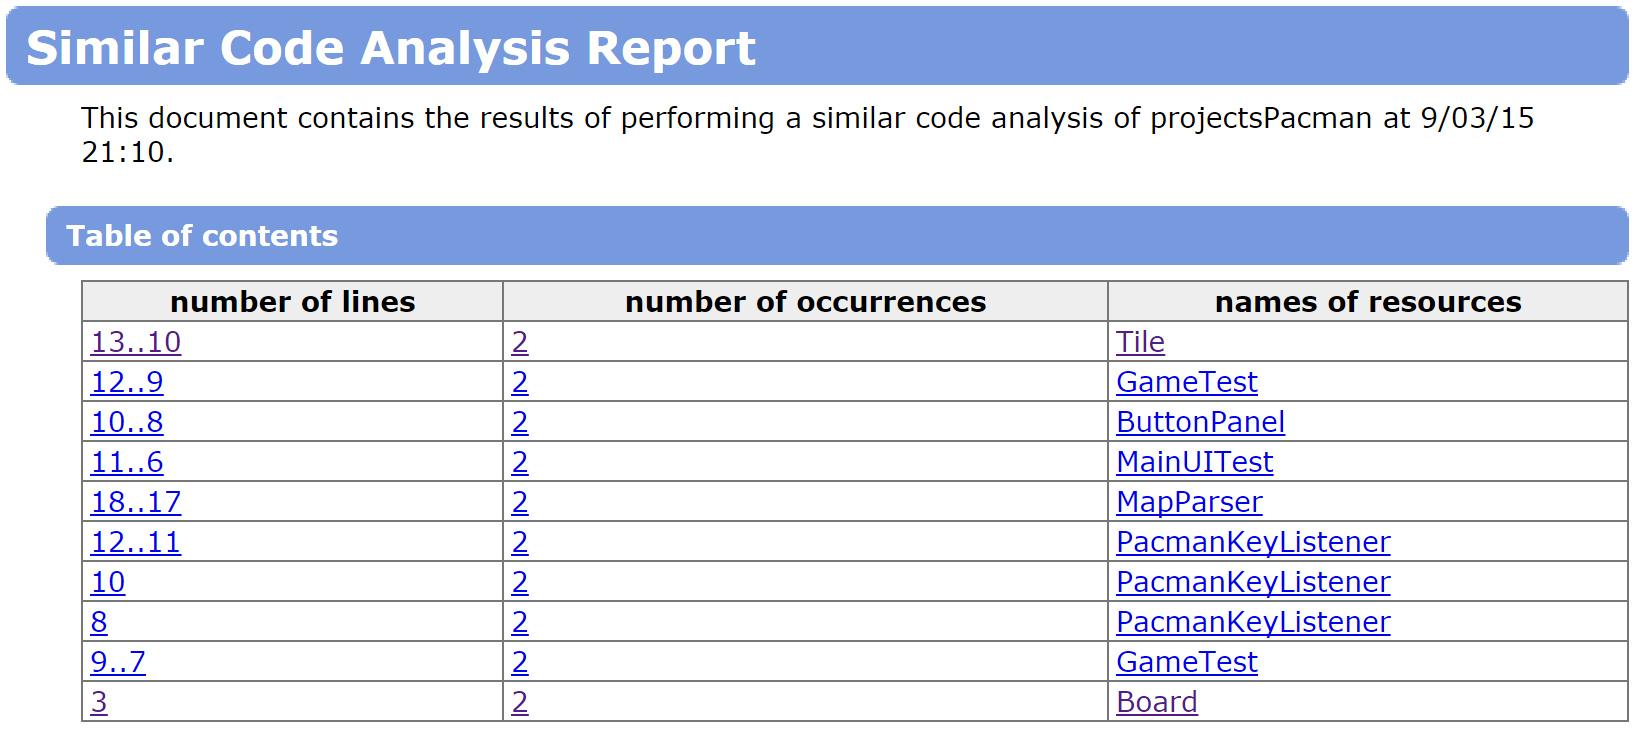
\includegraphics[width=\textwidth]{SimilarCode_00.png}
	\caption{\label{SimilarCode0}Résultat de l'analyse de "code dupliqué" par CodePro}
\end{figure}
Pour analyser cette métrique, nous avons utilisé le programme CodePro à partir de l'interface d'Eclipse ( Eclipse -> CodePro Tools -> Find Similar Code).\\
Nous pouvons observer sur la \labelfigure{SimilarCode0} que cet outil a détécté 10 blocs de code. Les figures de l'\annexe{SimilarCode} permettent de visualiser les différents blocs de code.
Les classes concernées sont : Tile.java, GameTest.java, ButtonPanel.java, MainUITest.java, MapParser.java, PacmanKeyListener.java, PacmanKeyListener.java, PacmanKeyListener.java,  GameTest.java, Board.java.\\
Ce résultat n'est pas bon, mais on peut observer que les blocs se trouvent chaque fois dans une même classe. Il sera donc probablement possible de créer des fonctions pour chacun de ces cas.

%%%%%%%%%%%%%%%%%%%%%%%%%%%%%%%%%%%%%%%%%%%%%%%%%%%%%%%%%%%%%%%%%%%%%%%%%%%%%%
\subsection{Dépendances cycliques}\label{dépendances}
Une dépendance cyclique peut-être appelée dépendance cyclique directe ou indirecte et elle a la même définition qu'il s'agisse de dépendances entre des projets, entre des packages ou entre des classes. Quand on a une dépendance directe, on a un élément X qui dépend d’un élément Y qui dépend lui-même de X. Contrairement à la dépendance cyclique indirecte où la situation dans laquelle on se trouve est tel que X dépend de Y, Y dépend de Z et Z dépend de X.\\
Du point de vue de la compilation, plus une dépendance est à haut niveau, plus elle est à traiter en priorité. En effet entre deux classes, ce n'est pas très grave et ça ne pose généralement pas de problème. Entre deux package c'est fortement déconseillé même s'il est généralement possible de compiler le projet. Par contre entre deux projets, l'issue est fatale puisque chaque projet doit-être compilé avant de pouvoir compiler l'autre.\\
Du point de vue de la maintenance, une dépendance d'un élément A à un élément B et vice-versa impose que pour pouvoir modifier A, il faut commencer par modifier B et pour pouvoir modifier B, il faut commencer par retravailler A. L'évolution de ces éléments est donc compliquée.\\
Pour pallier à ce genre de problème, plusieurs pistes sont possible : déplacer les éléments (les classes si le problème concerne deux packages ou la(les) méthode(s) si le soucis se situe entre deux classes), redécouper certains éléments (pour mieux associer les blocs de code aux éléments qui en ont besoin), regrouper les éléments (pour n'en former plus qu'un seul),... %piste de solution à l'adresse  :http://blog.developpez.com/wichtounet/p8723/jtheque/osgi_et_dependances_cycliques
\begin{figure}[!h]
	\centering
	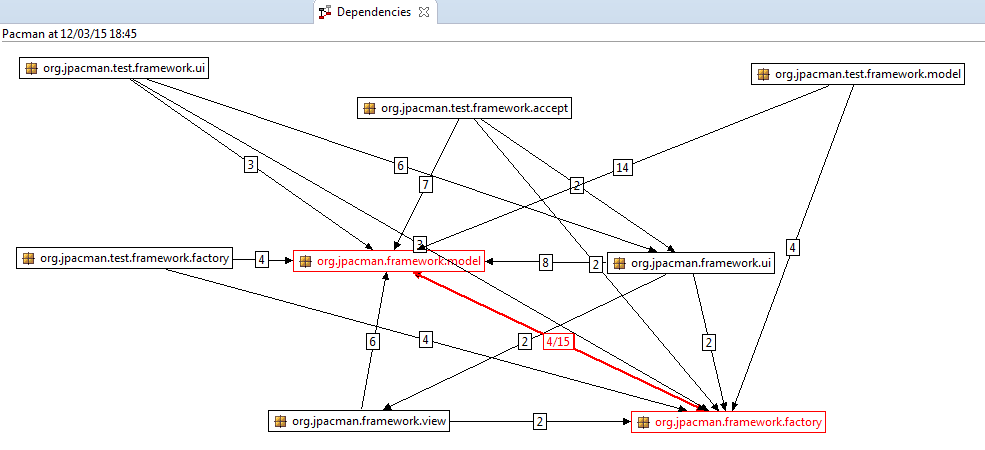
\includegraphics[width=\textwidth]{DependenciesPackages.png}
	\caption{\label{dependenciesPackage}Détail de l'analyse des dépendences cycliques des packages du projet.}
\end{figure}
\begin{figure}[!h]
	\centering
	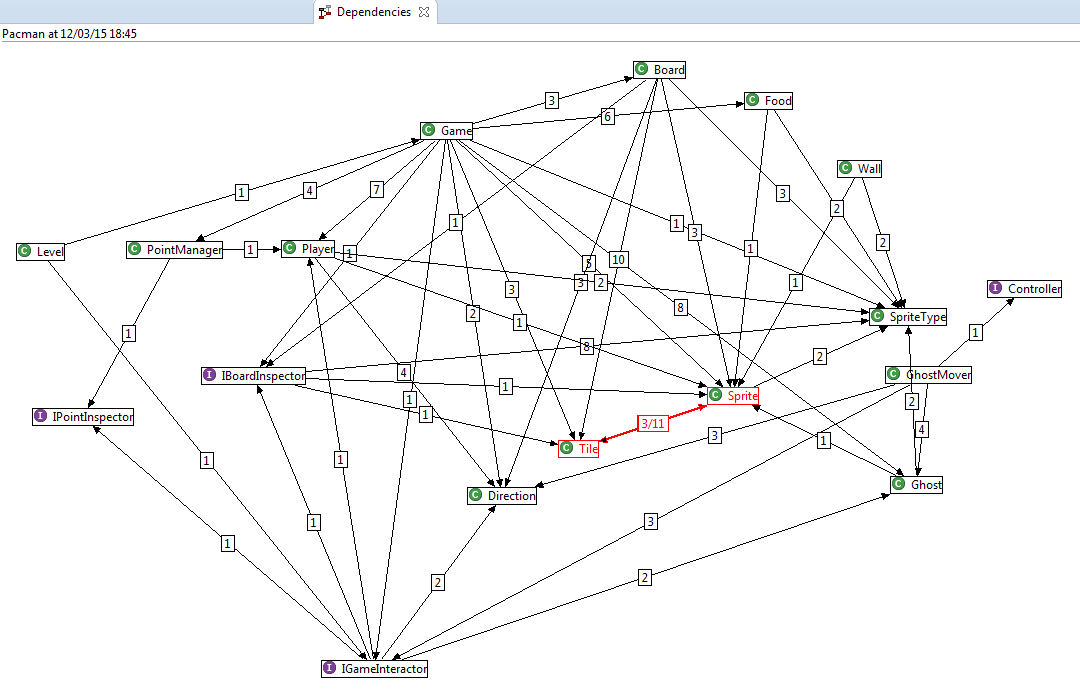
\includegraphics[width=\textwidth]{DependenciesModel.png}
	\caption{\label{dependenciesModel}Détail de l'analyse des dépendences cycliques du package Model.}
\end{figure}
Cet métrique a aussi été visualisée à partir de l'outil CodePro depuis Eclipse (Eclipse -> CodePro Tools -> Analyse Dependencies).
On peut observer sur la \labelfigure{dependenciesPackage} et la \labelfigure{dependenciesModel} qu'il existe des dépendances cycliques au sein du package "model" (entre les classes Sprite et Tile) et entre le package "model" et le package "factory".\\
L'\annexe{Dependencies} contient toutes les autres visualisations qui n'ont pas révélé de problème de dépendances.

%%%%%%%%%%%%%%%%%%%%%%%%%%%%%%%%%%%%%%%%%%%%%%%%%%%%%%%%%%%%%%%%%%%%%%%%%%%%%%
\subsection{Code inutile}\label{deadCode}
Du code inutile, aussi appelé "Dead Code", correspond à des lignes de code qui sont compilées mais qui ne sont jamais utilisées.\\
C'est fréquemment du code qui a été utile à une fonctionnalité et lorsque cette fonctionnalité a été supprimée, réécrite, déplacée,... ce code est resté. Le problème dans ce cas est que ça ralentit la compréhension du développeur lors de la lecture, ça gaspille des ressources au compilateur et lors de l'exécution.\\
La solution est généralement de supprimer ces lignes de code.
\begin{figure}[!h]
	\centering
	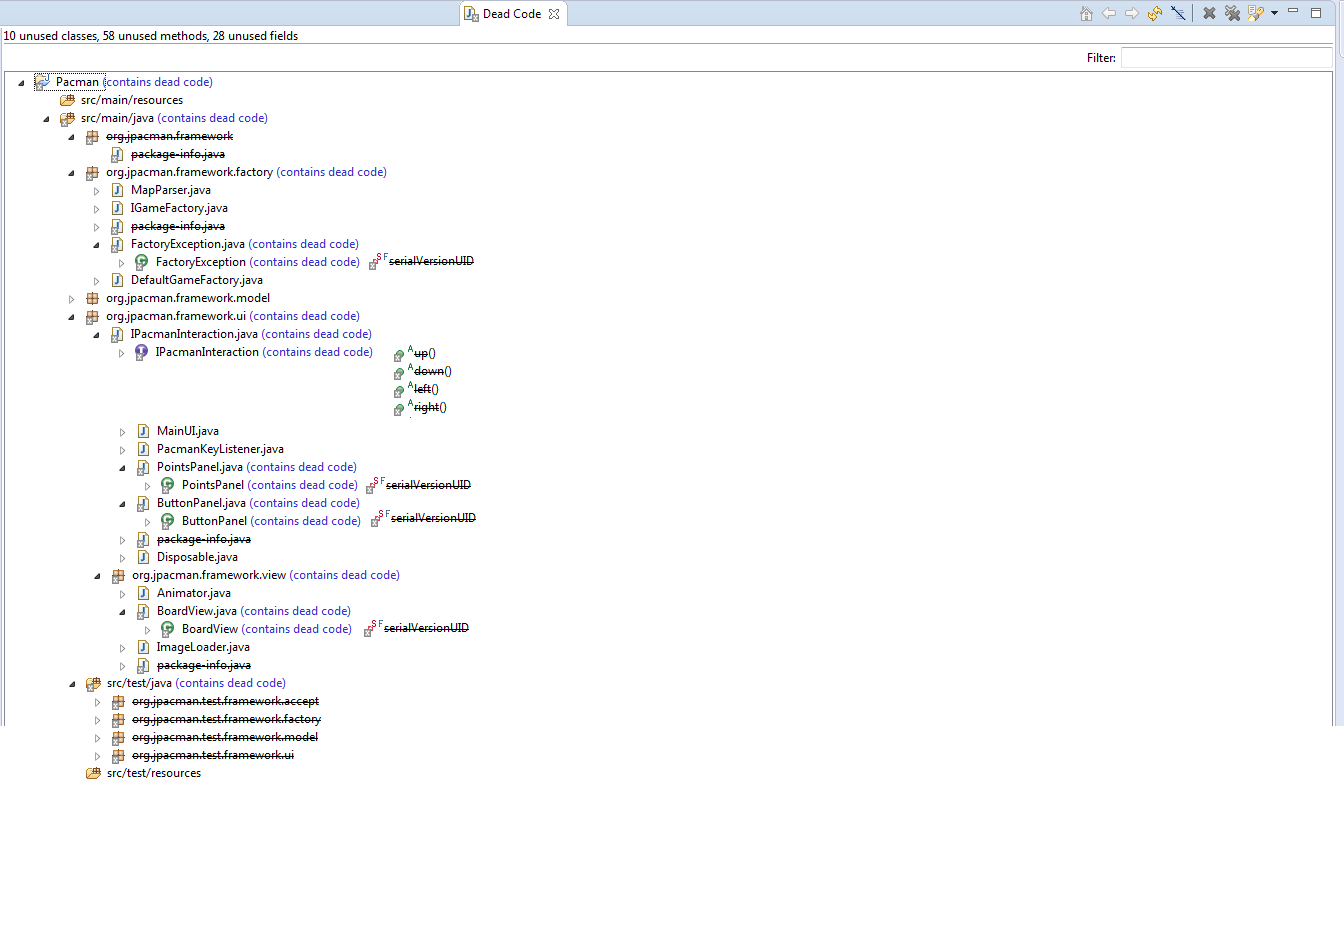
\includegraphics[width=\textwidth]{DeadCode.png}
	\caption{\label{deadcode}Détail de l'analyse des parties de code non utilisé lors de l'éxécution du programme.}
\end{figure}
L'outil utilisé reste CodePro depuis Eclipse (Eclipse -> CodePro Tools -> Find dead code).\\
Attention tout de même à ne pas tout supprimer sans réfléchir, en effet, on observe sur la \labelfigure{deadcode} que les packages contenant les tests sont considérés comme inutile. Ils le sont en effet lors de l'exécution du programme, mais ne le sont pas au bon développement du programme. Il en va de même pour les variables "serialVersionUID". Ces variables, bien que inutile lors de l'exécution, doivent être présentes dans les classes qui étendent (directement ou indirectement) la classe "Sérializable". Leur valeur est indispensable pour des applications qui transitent par le réseau mais leur existence ne peut causer aucun tort. Pour ce qui est des fichiers "package-info.java", ils sont à nouveau inutiles lors de l'exécution du code, mais permettent de contenir les commentaires contenant l'information relative au package en vue de la création de la javadoc. Ces fichiers sont donc à conserver (et à complêter dans certains cas).\\
L'analyse a aussi été effectuée par l'outil Code Inspector de IntelijIdea et donne d'autres résultats complémentaires. Ceux-ci font référence à des méthodes complètes qui ne sont jamais appelées.\\
La solution, la plus rapide, est simplement de supprimer ces méthodes. Seulement si lors d'une future amélioration, on se rend compte qu'elles auraient pu être nécessaire, on doit recommencer le travail. Une autre solution pourrait être de mettre ces fonctions en commentaire afin de ne pas devoir réécrire ces fonctions.\\
Les modifications à éffectuer, bien que nombreuses, sont donc mineures.

%%%%%%%%%%%%%%%%%%%%%%%%%%%%%%%%%%%%%%%%%%%%%%%%%%%%%%%%%%%%%%%%%%%%%%%%%%%%%%
\subsection{Javadoc}\label{javadoc}
La javadoc est une documentation standard au format HTML pour les programmes développés en JAVA. Elle est créée de façon automatique par la plupart des outils de développement en se basant sur les tags placés dans le code au dessus de la déclaration de chaque classe et de chaque méthode (pour la documentation des packages, elle se trouve dans les fichiers "paquage-info.java").
L'utiliser est un plus mais ne consiste en rien en une obligation (mais alors il sera tout de même fortement conseillé d'utiliser les commentaires classiques pour constituer un code suffisamment documenté à la compréhension).\\
Grâce à l'outil CodePro d'Eclipse, il a été observé (non illustré parce que toutes les classes sont à revoir) que en règle générale, les classes sont documentées. L'outil détecte bien quelques manquement, mais ce sont généralement l'un ou l'autre tag qu'il détecte manquant mais qui ne perturbe pas la compréhension ainsi que les classes DefaultGameFactory, Game, IBoardInspector, IPointInspector, Player et PointManager dont les méthodes ne sont pas commentées et les méthodes issues d'une interface (sous l'annotation "@Overhide").
%Code inspector de Intelijidea a repérer le tag @param sprite manquant à la ligne 233 de la fonction spriteImage(Sprite) de la calsse BoardVieuw du package org.jpacman.framework.view

%%%%%%%%%%%%%%%%%%%%%%%%%%%%%%%%%%%%%%%%%%%%%%%%%%%%%%%%%%%%%%%%%%%%%%%%%%%%%%
\subsection{Test unitaire}
Les tests unitaires permettent de vérifier le bon fonctionnement du programme en testant les lignes de codes du logiciel. C'est pourquoi, que dans cette section,une analyse est réalisée sur les différents tests unitaires en fesant un test de couverture.\\
Tout d'abord, lorsque les tests sont lancés (avec Intellij IDEA), tous les tests sont réussis sauf trois qui sont ignorés.\\
Ensuite, grâce à l'outil de couverture de test dans Intellij IDEA, il est possible de voir les méthodes testées et celles qui ne le sont pas. Les tableaux qui suivent montrent le résultat de la couverture de test.\\
Comme le montre le tableau \ref{Résumé de l'analyse de couverture}, l'analyse de couverture des tests montre que 96\% du code est couvert. Ce qui correspond à 90\% des méthodes et 88\% de lignes.\\
Des tests devrons être ajoutés pour couvrir et tester les méthodes dans la classe "MapParser". Ceux-ci permettent de voir si les exceptions sont bien lancées lorsqu'une map est mal encodée.\\
Après,l'analyse montre que les méthodes withFactory et withButtonPanel dans la classe MainUI ne sont pas testées.\\

De plus, les évènements du clavier, se trouvant dans la classe "PacmanKeyListener", ne sont pas testés et devront l'être. Tout comme pour les boutons "play", "stop" et "exit" se trouvant dans le ButtonPanel.\\ 

\begin{table}[!h]
\begin{tabular}{|l|l|l|l|}
\hline
Package & \ Classe,\% & \ Methode,\% & \ Ligne,\% \\
\hline
Toutes les classes & 96,6\% (28/29) & 90\% (198/220) & 88,3\% (704/797) \\
\hline
\end{tabular}
\caption{Résumé de l'analyse de couverture}
\label{Résumé de l'analyse de couverture}
\end{table}

Puis, le tableau \ref{Répartition de couverture des tests} montre plus précisément la répartition de couverture entre les différents packages.
Le tableau révèle que toutes les classes sont testées sauf une qui est la classe FactoryException se trouvant dans le package factory.
De plus, il souligne que la plus part des méthodes sont testées mais toutes ne le sont pas. 

\begin{table}[!h]
\begin{tabular}{|l|l|l|l|}
\hline
Package & \ Classe,\% & \ Methode,\% & \ Ligne,\% \\
\hline
org.jpacman.framework.factory & \ 66,7\% (2/3) & \ 84,2\% (16/19) & \ 75\% (69/92) \\
\hline
org.jpacman.framework.model & \ 100\% (13/13) & \ 93,5\% (87/93) & \ 96,1\% (273/ 284)) \\
\hline
org.jpacman.framework.ui & \ 100\% (8/8) & \ 82,9\% (63/76) & \ 81,3\% (226/278) \\
\hline
org.jpacman.framework.view & \ 100\% (5/5) & \ 100\% (32/32) & \ 95,1\% (136/143) \\
\hline

\end{tabular}
\caption{Répartition de couverture des tests}
\label{Répartition de couverture des tests}
\end{table}

%%%%%%%%%%%%%%%%%%%%%%%%%%%%%%%%%%%%%%%%%%%%%%%%%%%%%%%%%%%%%%%%%%%%%%%%%%%%%%
\subsection{Flux de conception}\label{designflaws}
A l'aide de l'outil InCode intégré à Eclipse, on peut entre-autre observer la conception du programme sur la \labelfigure{designflaws} dont la légende se trouve à l'\annexe{designflawsLeg}
\begin{figure}[!h]
	\centering
	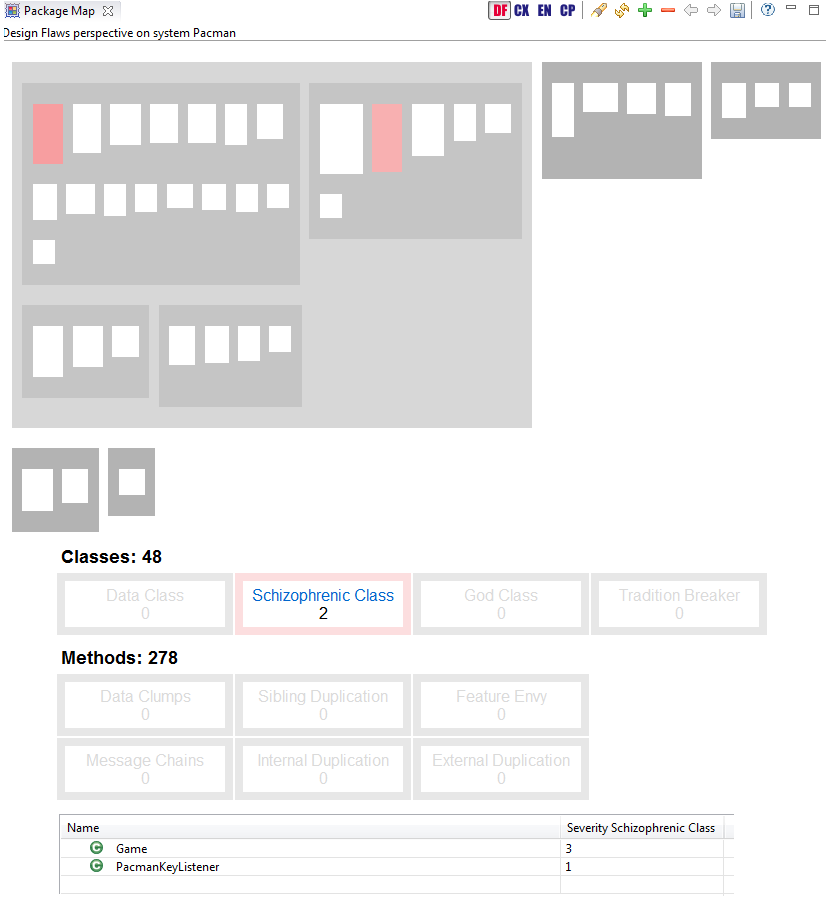
\includegraphics[width=\textwidth]{InCodeDesignFlaws.png}
	\caption{\label{designflaws}Analyse de la conception du programme (sa structure) par InCode.}
\end{figure}
La \labelfigure{designflaws} illustre donc que il n'y a pas de gros problèmes dans l'application(point de vue structure) cependant 2 classes ont tout de même un comportement inadéquat : Game et PacmanKeyListener. Ils sont répertoriées comme des classes schizophréniques.\\
Ces classes ont la particularité  d'être utilisées par des groupes disjoints de classes de clients utilisant des fragments disjoints de la classe.\\
Plusieurs solutions sont possible pour résoudre ce genre de problème :
\begin{itemize}
\item Regrouper les éléments qui sont utilisés par des groupes disjoints de clients et en faire 2 classes distinctes.
\item Revoir l'accessibilité des éléments qui la contiennent.
\item Regardez l'aperçu de la vue "couplage" pour identifier toutes les dépendances basées sur les appels entre la classe courante et les classes externes.
\end{itemize}

%%%%%%%%%%%%%%%%%%%%%%%%%%%%%%%%%%%%%%%%%%%%%%%%%%%%%%%%%%%%%%%%%%%%%%%%%%%%%%
\subsection{Complexité}
A l'aide de l'outil InCode intégré à Eclipse, on peut entre-autre observer la complexité de l'application sur la \labelfigure{complexity} dont le détail de la légende se trouve à l'\annexe{complexityLeg}
\begin{figure}[!h]
	\centering
	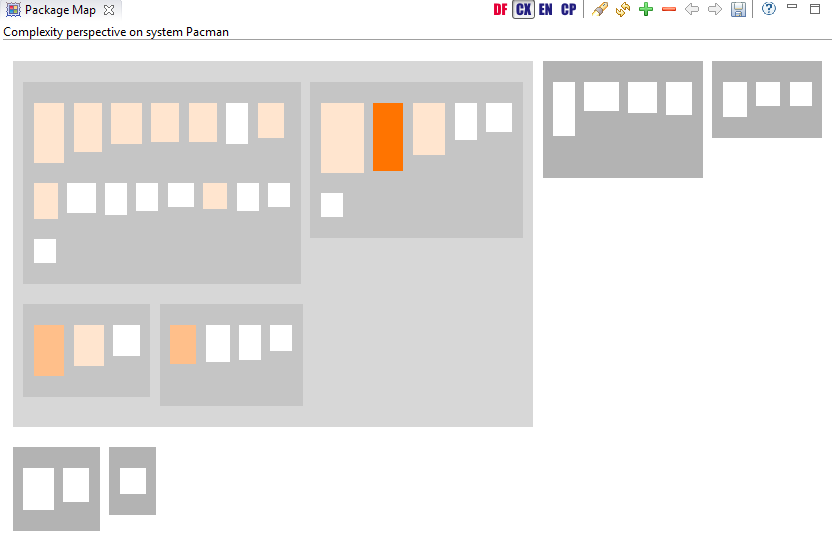
\includegraphics[width=\textwidth]{InCodeComplexity.png}
	\caption{\label{complexity}Analyse de la complexité par InCode.}
\end{figure}
Cette figure met en avant la classe PacmanKeyListener qui encourt la plus forte complexité et met un attention sur les classes BoardView et MapParser (à cause de leur grand nombre d'attributs).

%%%%%%%%%%%%%%%%%%%%%%%%%%%%%%%%%%%%%%%%%%%%%%%%%%%%%%%%%%%%%%%%%%%%%%%%%%%%%%
\subsection{Encapsulation}
A l'aide de l'outil InCode intégré à Eclipse, on peut entre-autre observer la complexité de l'application sur la \labelfigure{encapsulation} dont le détail de la légende se trouve à l'\annexe{encapsulationLeg}
\begin{figure}[!h]
	\centering
	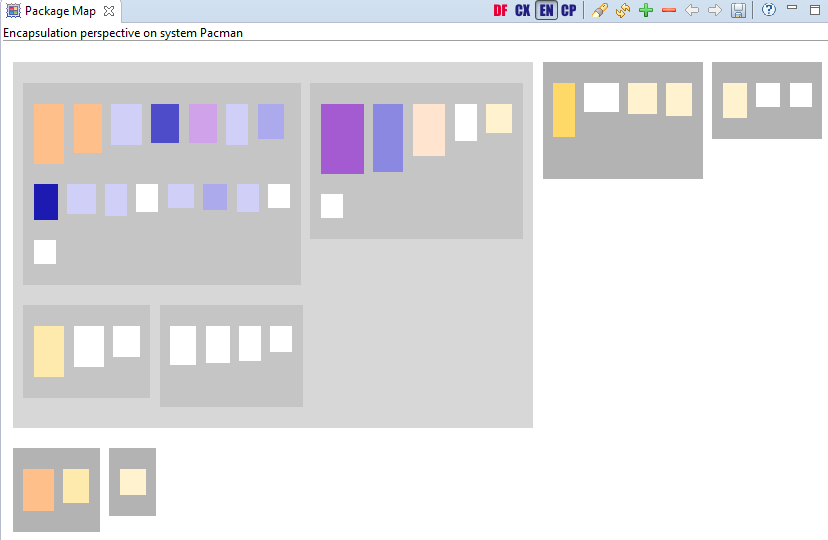
\includegraphics[width=\textwidth]{InCodeEncapsulation.png}
	\caption{\label{encapsulation}Analyse de la complexité par InCode.}
\end{figure}
Cette figure contient beaucoup d'informations, nous en retiendrons quelques unes : 
\begin{itemize}
\item La classe "MainUI" a beaucoup de clients (c'est-à-dire beaucoup d'autres classes qui accèdent aux données publiques de cette classes) dont les principaux sont "PacmanKeyListener" et "IGameInteractor". On ne sait rien concernant le nombre de fournisseurs (c'est-à-dire beaucoup de données publiques d'autres classes auxquelles celle-ci accède) sauf qu'il est inférieur au nombre de clients.
\item La classe "Player" n'a aucun fournisseur et a beaucoup de clients dont les principaux sont "Game" et "BoardView".
\item La classe "Sprite" n'a aucun fournisseur et a beaucoup de clients dont les principaux sont "Game", "Board" et "Tile".
\item Les classes telles que "Ghost", "Controller", "Wall", "ImageLoader", "Animator", "MapParser", "IGameFactory", "FactoryException", "IPacmanInteraction" et "Disposable" n'ont ni clients ni fournisseurs.
\end{itemize}

%%%%%%%%%%%%%%%%%%%%%%%%%%%%%%%%%%%%%%%%%%%%%%%%%%%%%%%%%%%%%%%%%%%%%%%%%%%%%%
\subsection{Couplage}
A l'aide de l'outil InCode intégré à Eclipse, on peut entre-autre observer la complexité de l'application sur la \labelfigure{coupling} dont le détail de la légende se trouve à l'\annexe{couplingLeg}
\begin{figure}[!h]
	\centering
	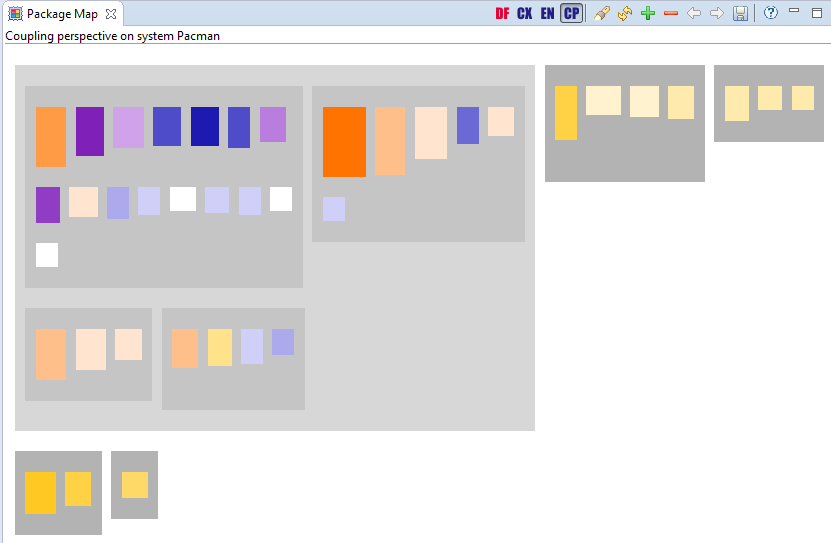
\includegraphics[width=\textwidth]{InCodeCoupling.png}
	\caption{\label{coupling}Analyse de la complexité par InCode.}
\end{figure}
Cette \labelfigure{coupling} contient aussi beaucoup d'informations, nous en retiendrons quelques unes : 
\begin {itemize}
\item La classe "MainUI" a beaucoup de fournisseurs\footnote{>provider} (c'est-à-dire beaucoup de méthodes publiques d'autres classes auxquelles celle-ci accède) dont les principaux sont "GhostMover", "IGameInteractor", "Level", "BoardView", "Animator", "PacmanKeyListener", "ButtonPanel" et "PointsPanel". On ne sait rien concernant le nombre de clients (c'est-à-dire beaucoup d'autres classes qui accèdent aux méthodes publiques de cette classes) sauf qu'il est inférieur au nombre de clients.
\item La classe "Tile" n'a aucun fournisseur et beaucoup de clients dont les principaux sont "Game", "Board" et "Sprite".
\item La classe "Board" a beaucoup de clients dont les principaux sont "Game", "MapParser" et "DefaultGameFactory". On ne sait rien concernant le nombre de fournisseurs sauf qu'il est inférieur au nombre de clients et que les principaux sont "Sprite" et "Tile".
\end{itemize}

%%%%%%%%%%%%%%%%%%%%%%%%%%%%%%%%%%%%%%%%%%%%%%%%%%%%%%%%%%%%%%%%%%%%%%%%%%%%%%
\subsection{Pyramide des métriques}
A l'aide de l'outil InCode intégré à Eclipse, on peut entre-autre observer les valeurs de l'application sur la \labelfigure{pyramid} dont le détail de la légende se trouve à l'\annexe{pyramidLeg}.
\begin{figure}[!h]
	\centering
	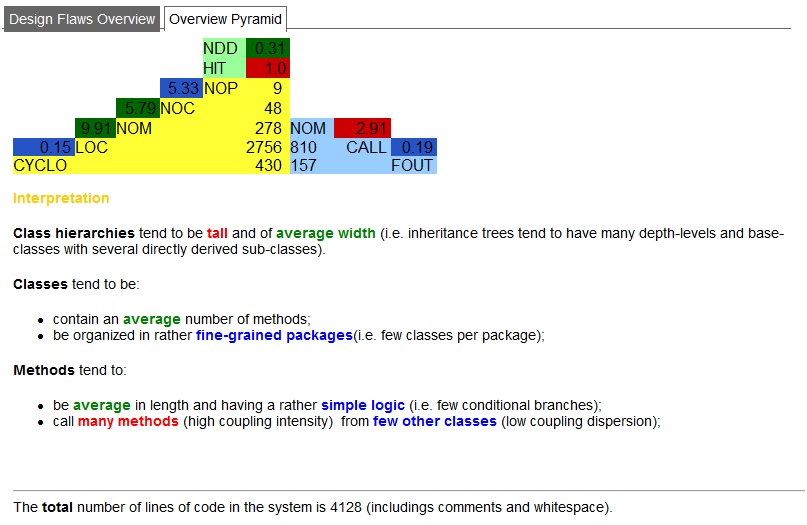
\includegraphics[width=\textwidth]{InCodePyramid.png}
	\caption{\label{pyramid}Pyramide des valeurs calculées par InCode.}
\end{figure}
Comme le précise l'interprétation de la \labelfigure{pyramid}, l'arbre que constitue les classes est grand et étroit.\\
Les classes ont tendance à contenir un nombre moyen de méthodes et à être organisé avec quelques classes par paquet.\\
Les méthodes tendent à être longue et avec une logique assez simple et à appeler de nombreuses méthodes (à forte intensité de couplage) de quelques autres classes (à faible dispersion de couplage).

\clearpage
%%%%%%%%%%%%%%%%%%%%%%%%%%%%%%%%%%%%%%%%%%%%%%%%%%%%%%%%%%%%%%%%%%%%%%%%%%%%%%
\subsection{Métriques}
Grace à l'outil de calcul des métriques d'Eclipse, on peut observer les résulats présent à la \labelfigure{métrique0}, la \labelfigure{métrique1} et la \labelfigure{métrique2}.\\
\begin{figure}[!h]
	\centering
	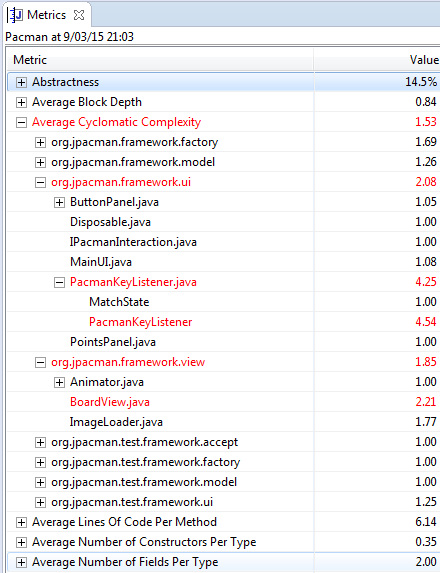
\includegraphics[height=\textheight]{Metrique0.png}
	\caption{\label{métrique0}Détails de l'analyse des métriques du projet (partie 1).}
\end{figure}
\begin{figure}[!h]
	\centering
	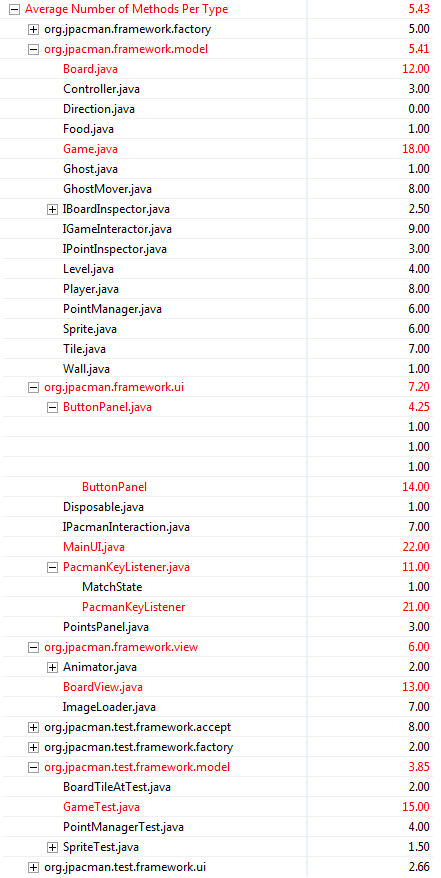
\includegraphics[height=\textheight]{Metrique1.png}
	\caption{\label{métrique1}Détails de l'analyse des métriques du projet (partie 2).}
\end{figure}
\begin{figure}[!h]
	\centering
	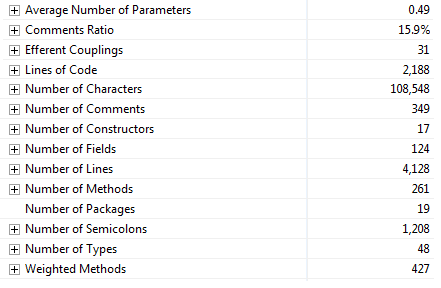
\includegraphics{Metrique2.png}
	\caption{\label{métrique2}Détails de l'analyse des métriques du projet (partie 3).}
\end{figure}
\subsubsection{Complexité cyclique moyenne}
Il s'agit de la moyenne de la complexité cyclomatique de chacune des méthodes. La complexité cyclomatique d'une méthode unique est une mesure du nombre de chemins distincts de l'exécution dans le procédé. Elle est mesurée par l'ajout d'une voie pour la méthode avec chacun des chemins créés par des instructions conditionnelles (telles que "if" et "for") et les opérateurs (tels que "? :").
\begin{figure}[!h]
	\centering
	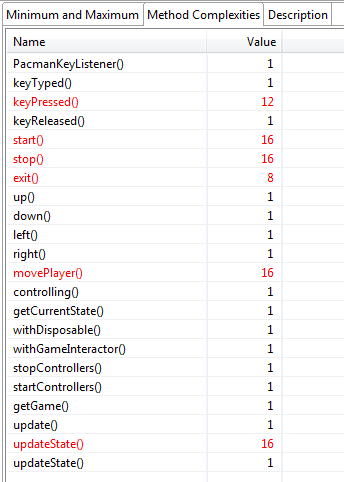
\includegraphics[width=\textwidth]{ACC_PacmanKeyListener.png}
	\caption{\label{ACC1}Détails de l'analyse de la complexité cyclique de la classe "PacmanKeyListener".}
\end{figure}
\begin{figure}[!h]
	\centering
	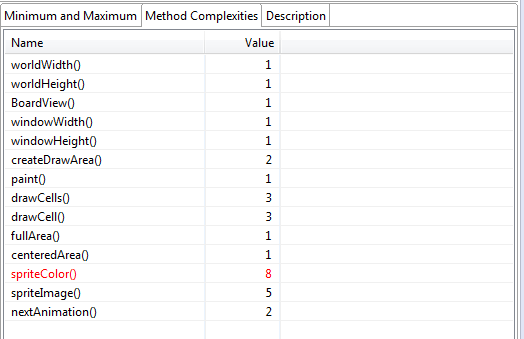
\includegraphics[width=\textwidth]{ACC_BoardView.png}
	\caption{\label{ACC2}Détails de l'analyse de la complexité cyclique de la classe "BoardView".}
\end{figure}
Pour chacun des cas illustrés dans la \labelfigure{ACC1} et la \labelfigure{ACC2}, il sera nécessaire lors du refactoring (voir \refsection{sec:etape3} ) d'analyser et de voir s'il sera possible de la diminuer.


\subsubsection{Nombre moyen de méthodes par type}
C'est la moyenne du nombre de méthodes définies pour chaque classe.
On remarque que certaines classes ont trop de méthodes, en particulier les classes "Game", "ButtonPanel", "MainUI", "PacmanKeyListener" et "BoardView". \\
Lors d'une analyse précédente (voir section \ref{designflaws} il avait été observé que les classes "Game" et "PacmanKeyListener" était schizophréniques. Le problème se résolvera donc probablement naturellement lors du traitement de ce problème. Pour ce qui est des autres classes, il sera nécéssaire lors du refactoring d'étudier l'utilité de chacune des méthodes et d'aviser au cas par cas le travail à effectuer sur chacune.

\clearpage
%%%%%%%%%%%%%%%%%%%%%%%%%%%%%%%%%%%%%%%%%%%%%%%%%%%%%%%%%%%%%%%%%%%%%%%%%%%%%%
\subsection{Audit}
Cet intitulé reprend tous les problèmes et les erreurs de code tel que les erreurs non capturées, la sérialisation les imports inutiles, les droits d'accès,...\\
Voici celles détectées par l'outil CodePro d'Eclipse : 
\begin{figure}[!h]
	\centering
	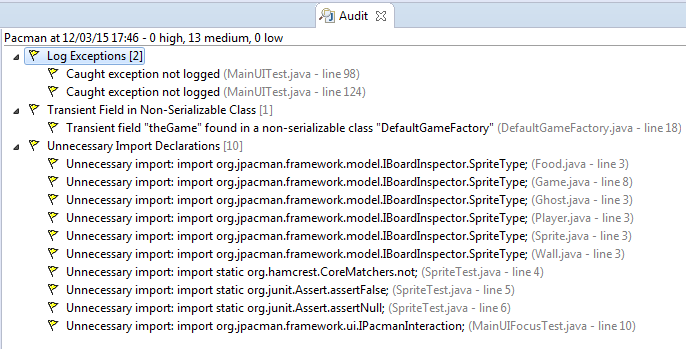
\includegraphics[width=\textwidth]{Audit.png}
	\caption{\label{Audit}Détail de l'analyse d'audit faite par Eclipse.}
\end{figure}

\subsubsection{Erreur non capturée}
Il s'agit de morceaux de code à risque (qui peuvent provoquer l'arrêt du programme avec une erreur fatale) qui n'est pas protégé.
Ici, les deux cas repérés sont encadrés par un bloc "try...catch" mais ils ne capturent qu'un seul type d'exception. Pour résoudre ce problème il suffira d'ajouter un second bloc "catch" qui prend en charge l'ensemble des autres exceptions.

\subsubsection{Sérialisation}
Un objet est sérialisable quand il implémente la classe "Serializable". Au sein d'un tel objet, tous les éléments doivent, par défaut, pouvoir l'être aussi. Dans le cas contraire, une variable globale peut-être qualifée avec le mot clé "`transient"` pour déclarer cette variable non sérialisable.
Dans ce cas-ci, l'objet DefaultGameFactory n'implémente pas la classe "Serializable" donc il n'y a aucune raison de déclarer une variable "transient".

\subsubsection{Import inutile}
Les imports sont les premières lignes d'une classe. Ils permettent d'informer au compilateur d'où viennent les méthodes, les objets,... utilisés qui ne sont pas créés au sein de la classe courante.
Egalement repris plus loin dans les warnings d'Eclipse, les classes comportent plusieurs imports qui ne sont jamais utilisés.
La meilleur solution est simplement de les supprimer.\\
Ceux détectés par l'outil Code Inspector d'IntelijIdea  se trouve à la \labelfigure{Audit}. 
\begin{figure}[!h]
	\centering
	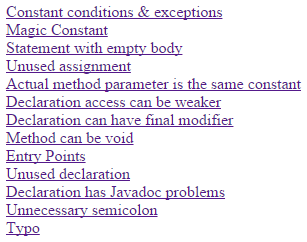
\includegraphics[width=\textwidth]{AuditII.png}
	\caption{\label{Audit}Détail de l'analyse d'audit faite par IntelijIdea.}
\end{figure}

\subsubsection{Droit d'accès}
Chaque élément d'un code (classe, sous-classe, méthode, variable,...) est qualifié d'un mot-clé qui permet de définir l'accessibilité tel que (pour une variable globale ou une méthode\footnote{un descriptif similaire peut-être fait pour une classe}): 
\begin{itemize}
\item public : \\
- Est accessible dans la classe\\
- Peut être accessible depuis une autre classe du package où elle se trouve.\\
- Peut être accessible depuis n'importe quelle classe extérieure au package.
\item protected :\\
- Est accessible dans la classe\\
- Peut-être accessible depuis une autre classe du package où elle se trouve (et des classes enfents).\\
- N'est pas accessible depuis n'importe quelle classe extérieure au package.
\item private :\\
- est accessible dans la classe\\
- Ne peut pas être accessible depuis une autre classe du package où elle se trouve.\\
- N'est pas accessible depuis n'importe quelle classe extérieur au package.
\end{itemize}
Une mauvaise pratique est de tout mettre en publique. Ca permet une vue d'ensemble sur son programme mais implique parfois certaines erreurs d'utilisation.\\
Ce n'est donc pas un problème grave à l'heure actuelle puisque le jeu fonctionne correctement mais lors de l'ajout de fonctionnalités cela peut le devenir.

\subsubsection{Optimisation}
En java, une variable qui ne doit pas être modifiée pendant le temps d'une exécution peut-être qualifiée avec le mot-clé "final". Ceci permet d'optimiser le code et de ne pas être confronté à une mauvaise utilisation de la variable par la suite.

\subsubsection{Restructuration}
Cet outil informe que la fonction "public int addPoints(int)" de la classe "org.jpacman.framework.model.Player" retourne une valeur qui n'est jamais utilisée et qui dont pourrait être transformée en "public void addPoints(int)".\\
Cette modification est à étudier avant d'agir pour vérifier s'il n'est pas nécéssaire pour une utilisation postérieur de garder cette valeur de retour.\\
Il informe aussi que deux autres fonctions reçoivent toujours la même valeur dans leur paramètre et que donc cette valeur pourrait devenir une constante.\\
Chacun des cas sera à étudier pour savoir si cette information est disponible à la méthode et que celle-ci doit alors être refactorée ou si elle a été mise en paramètre en vue d'une amélioration future.

\subsubsection{Code inutile}
Ce sujet a déjà été traité plus haut (Voir \ref{deadCode}).

\subsubsection{Javadoc}
Ce sujet a déjà été traité plus haut (Voir \ref{javadoc}).

\subsubsection{Caractère inutile}
Ce sont des éléments du code qui sont sous-entendu par le reste de l'architucture du code.\\
Dans ce projet, un seul cas a été resencé, il s'agit d'un ";" dans la classe "IBoardInspector" du package "org.jpacman.framework.model". Lors du refactoring, il suffira de le retirer.

\subsubsection{Typographie}
Les problèmes de typographies reprennent les erreurs de formatage des différents éléments. Ce ne sont que des erreurs de conventions parce que elles ne changent en rien le comportement de l'application. Cependant, un bon respect des conventions permet une meilleur compréhension lors d'une relecture, d'une modification, de l'étude du code par un nouveau développeur sur le projet,...\\
L'outil Code Inspector intégré à IntelijIdea a permis d'en recenser plusieurs. A l'étude de celle-ci, il a été observé qu'elles sont souvent dans les commentaires. Exemple, dans le fichier "GhostMover.java" du package "org.jpacman.framework.model", entre la ligne 28 et la ligne 30, le mot "randomizer" a été identifié avec une majuscule dans le commentaire et sans majuscule dans les lignes de code.\\ \\
Il est important de signaler aussi, que l'outil Eclipse soulève certaines attentions à l'aide de "warnings".\\
Les types d'erreurs sont : 
\begin{itemize}
\item Empty block should be documented x2
\item Javadoc: Missing comment for public declaration x 51
\item Redundant specification of type arguments <...> x6
\item The import ... is never used x4
\item The method ... of type ... should be tagged with @Override since it actually overrides a superinterface method x13
\item The parameter ... is hiding a field from type ... x 7
\end {itemize}
Leurs emplacements : \\
\begin{table}[!h]
\begin{tabular}{|l|l|l|l|}
\hline
Package & \# warning & Classe & \# warnings \\
\hline
/main/java/.../model & 60 & Game.java & 15 \\
&& IBoardInspector.java & 13 \\
&& Direction.java & 8 \\
&& Player.java & 7 \\
&& Board.java & 4 \\
&& IPointInspector.java & 3 \\
&& PointManager.java & 3 \\
&& Tile.java & 3 \\
&& GhostMover.java & 2 \\
&& Sprite.java & 1 \\
&& Food.java & 1 \\
\hline
/main/java/.../ui & 15 & ButtonPanel.java & 8 \\
&& PacmanKeyListener.java & 5 \\
&& MainUI.java & 2 \\
\hline
/test/java/.../model & 5 & SpriteTest.java & 5 \\
\hline
main/java/.../factory & 2 & MapParser.java & 2 \\
\hline
/test/java/.../ui & 1 & MainUIFocusTest.java & 1 \\
\hline
\end{tabular}
\caption{Emplacement des "warnings" signalé par Eclipse}
\label{warnings}
\end{table}

%%%%%%%%%%%%%%%%%%%%%%%%%%%%%%%%%%%%%%%%%%%%%%%%%%%%%%%%%%%%%%%%%%%%%%%%%%%%%%
\subsection{Profilage}
\begin{figure}[!h]
	\centering
	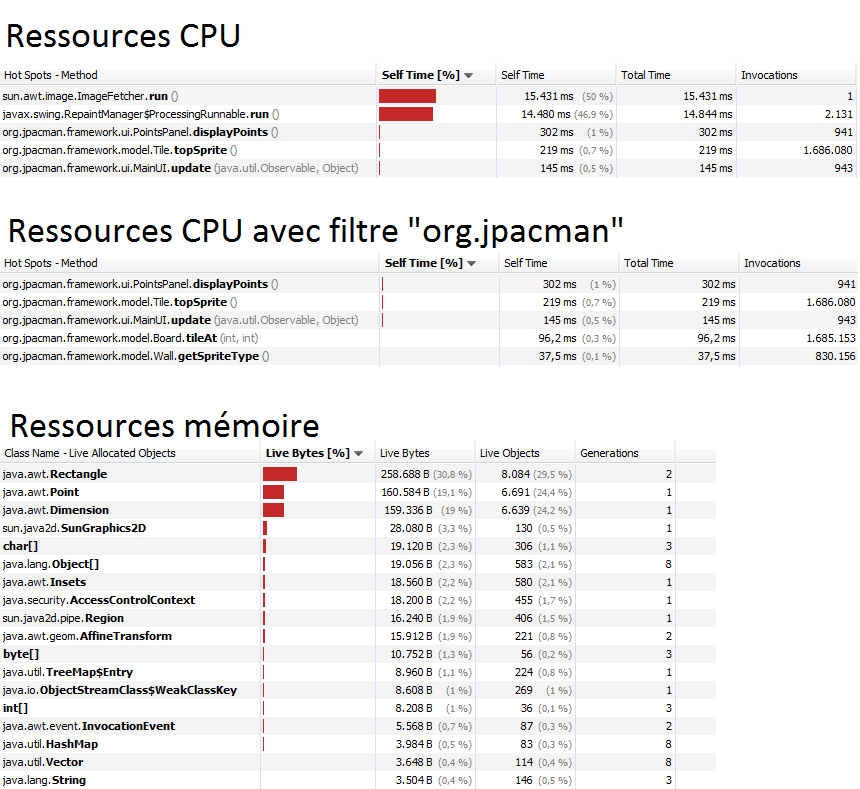
\includegraphics[width=\textwidth]{Profilage.png}
	\caption{\label{profilage}Détail de l'analyse des ressources CPU et mémoire par VisualVM.}
\end{figure}
\subsubsection{Ressources CPU}
Comme visible sur la \labelfigure{profilage}, c'est la chargement des images qui prend le plus de temps. Ceci étant une fonction externe au projet, il n'est pas possible d'y effectuer une modification. La méthode, sur laquelle il serait peut-être possible d'effectuer des changements, s'appelle "displayPoint" de la classe "org.jpacman.framework.ui.PointsPanel". Celle-ci calcule à chaque mise-à-jour de l'affichage le nombre de points déjà récoltés sur le nombre de points totaux. Cependant, la fonction est simple et ne prend en elle-même que très peu de temps. Ce qui pénalise est le nombre d'appel, qui lui ne peut pas être modifié puisqu'il est est necéssaire que ce score soit toujours à jour. \\
Il n'est donc probablement pas possible d'accélérer l'application.

\subsubsection{Consommation mémoire}
Les ressources mémoires utilisées par l'application sont visible dans la seconde moitié de la \labelfigure{profilage}. Les observations ne sont pas nombreuses si ce n'est que l'utilisation de la mémoire concerne majoritairement l'affichage et les éléments graphiques de l'application. A moins donc de diminuer la qualité ou la vitesse de rafraichissement (ce qui est fortement déconseillé), il n'y a pas grand chose à faire.


%%%%%%%%%%%%%%%%%%%%%%%%%%%%%%%%%%%%%%%%%%%%%%%%%%%%%%%%%%%%%%%%%%%%%%%%%%%%%%
\subsection{Conclusion}
Suite à cette analyse, il est evident de constater que ce code n'est pas parfait, cependant, dans l'ensemble il est correctement écrit, bien structuré, généralement commenté et facilement compréhensible. De ce point de vue il est donc normal d'estimer que certe certaines améliorations sont conseillées tel que les dépendances cycliques entre les packages et l'ajout de test unitaire mais dans l'ensemble, c'est un bon projet qui devrait être facile à maintenir et à poursuivre.

%%%%%%%%%%%%%%%%%%%%%%%%%%%%%%%%%%%%%%%%%%%%%%%%%%%%%%%%%%%%%%%%%%%%%%%%%%%%%%%%%%
\newpage
\clearpage
\section{Etape 2 : Ajout de tests unitaires}\label{sec:etape2}
Maintenant que l'analyse est terminée et avant de commencer à corriger les problèmes soulevé, il convient d'en vérifier le comportement à l'aide de test unitaire. Ces tests vont permettre de créer des scénario avec tous les cas de figure pour tester lors exécution.
Les test unitaire permettent ainsi de s'assurer que les modifications apporté au code source ne modifieront pas le comportement du logiciel.
%Tests  Eclipse -> Coverage As -> JUnit Test : La figure \annexe{coverage} montre que le projet est couvert à $68.3 \%$ avec en particulier, $63.5\%$ pour la package \emph{main} et $83.7\%$ pour le package \emph{test}.  Il est donc important d'ajouter des tests sur les classes : FactoryException, Board, Sprite et PacmanKeyListener qui sont sous le seuil des $50 \%$ de couverture.
Tout d'abord, les tests qui étaient ignorés ont été rajoutés. Et les deux méthodes, se trouvant dans la classe MainUI, qui n'etait pas couverte, le sont maintenant.\\
Ensuite, des tests ont été ajoutés dans la nouvelle classe MapParserTest\footnote{Les test sont trié. Chaque classe du package "src.main.java.org.jpacman.framework.*" est reliée à la classe de même nom suivit du mot-clé "Test" dans le package "src.test.java.org.jpacman.test.framework.*".}. Ils permettent de vérifier que lorsqu'une mauvaise map est mal encodé, les exceptions se lancent bien. Par exemple, lorsq'une map est vide, contient de mauvais caractères, n'a pas une taille "rectiligne",...\\
Après, des tests ont été rajoutés pour voir si les boutons "play", "stop" et "exit" fonctionnent correctement. Pour cela, un premier test regarde que le joueur ne peut pas bouger lorsque que le bouton pause est appelé et un autre test vérifie que la fenêtre se ferme bien lorsque le bouton "exit" est utilisé.\\
Enfin, des tests ont été rajoutés pour vérifier le bon fonctionnement des racourcis clavier. C'est-à-dire que les tests regardent que l'action à effectuer est bien réalisée. Donc les touches haut, bas, gauche, droite, x,s,q sont testées.\\
Pour conclure, le tableau \ref{Résumé de l'analyse de couverture après l'ajout de tests} montre bien que toutes les classes et presque toutes les méthodes sont couvertes. Les méthodes qui ne sont pas couvertes sont des accesseurs (getters et setters) et des méthodes toString().\\
Grâce aux tests ajoutés, la couverture du code est nettement améliorée.\\

\begin{table}[!h]
\begin{tabular}{|l|l|l|l|}
\hline
Package & \ Classe,\% & \ Methode,\% & \ Ligne,\% \\
\hline
Toutes les classes & 100\% (29/29) & 96,4\% (212/220) & 96,5\% (769/797) \\
\hline
\end{tabular}
\caption{Résumé de l'analyse de couverture après l'ajout de tests}
\label{Résumé de l'analyse de couverture après l'ajout de tests}
\end{table}
%Tests  Eclipse -> Coverage As -> JUnit Test : La figure \annexe{coverage} montre que le projet est couvert à $68.3 \%$ avec en particulier, $63.5\%$ pour la package \emph{main} et $83.7\%$ pour le package \emph{test}. Il est donc important d'ajouter des tests sur les classes : FactoryException, Board, Sprite et PacmanKeyListener qui sont sous le seuil des $50 \%$ de couverture.

%%%%%%%%%%%%%%%%%%%%%%%%%%%%%%%%%%%%%%%%%%%%%%%%%%%%%%%%%%%%%%%%%%%%%%%%%%%%%%%%%%
\newpage
\section{Etape 3 : Refactoring en vue d'améliorer la qualité\\Etape 4 : Analyse de la qualité du logiciel} \label{sec:etape3} \label{sec:etape4}
Maintenant que l'ensemble du code est couvert par les test, il est réaliste de vouloir modifier le code pour l'améliorer. Grace aux différents tests, on peut garantir une certaine stabilité du logiciel et que celui-ci continuera à fonctionner. Après chaque modification, un lancement de l'ensemble des tests sera réalisé pour pouvoir éventuellement faire marche arrière si la modification rétrograde le logiciel.\\
Cette section va reparcourir chacune des sous-sections de la section \refsection{sec:etape1} et détaillera les chagements réalisés et les changements non réalisés. Pour une meilleur clarté, l'analyse de la qualité du logiciel sera détaillée simultanément\footnote{L'analyse a été réalisée une fois tout le refactoring réalisé}.\\
N.B. : Les analyses et le refactoring ne concernent pas les tests.

%\subsection{Enoncé}Avec les tests unitaires ajoutés dans l'étape précédente, vous pouvez vérifier automatiquement (jusqu'à un certain point) la préservation du comportement du logiciel. Réalisez les modifications nécessaires à l'amélioration de la qualité et la structure du logiciel. Vos ressources et votre temps étant limités, commencez par établir les modifications devant être réalisées en priorité. Sur base de quels critères réalisez-vous cette priorisation ? Refactorisez progressivement votre code, en vous assurant systématiquement que tous les tests déjà présents s'exécutent avec succès. Souvenez-vous que vos modifications doivent améliorer la qualité du code, et non étendre ou modifier le comportement du logiciel.
%%%%%%%%%%%%%%%%%%%%%%%%%%%%%%%%%%%%%%%%%%%%%%%%%%%%%%%%%%%%%%%%%%%%%%%%%%%%%%%%%%%%
\subsection{Code dupliqué}\label{codeduplique_refact}
Il est important de traiter cette section parce que pour la maintenance d'un projet, il est impératif de ne pas devoir effectuer un chagement plusieurs fois et risquer de ne pas effectuer le changement quelque part.
\begin{figure}[!h]
	\centering
	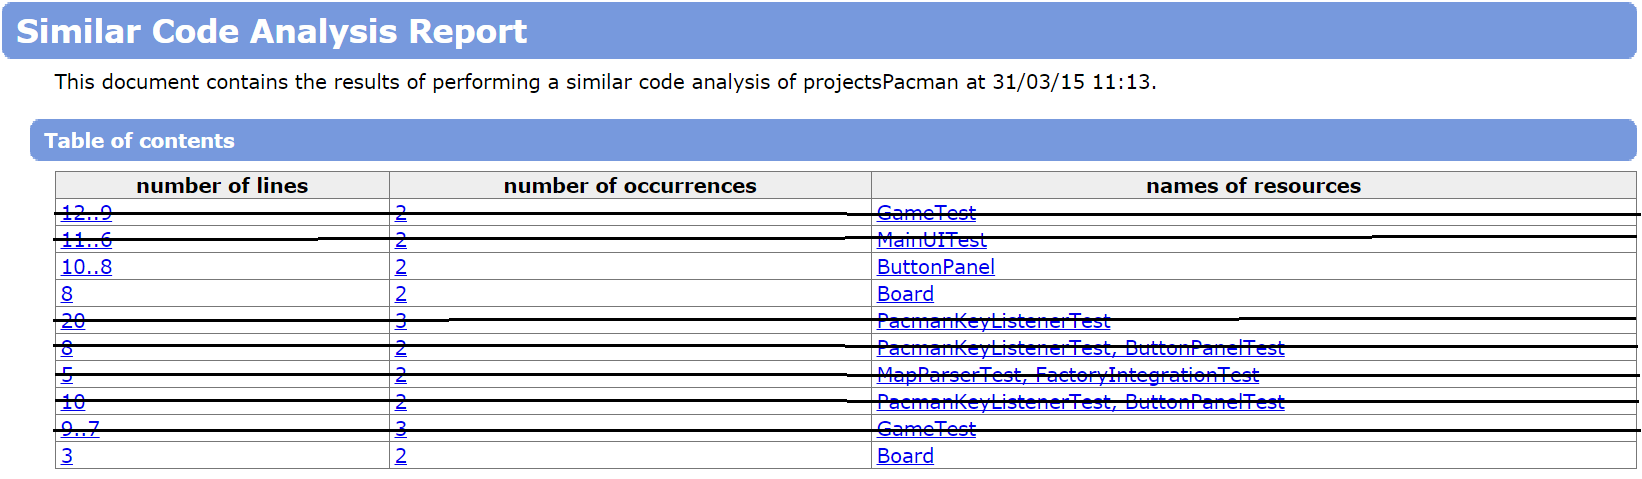
\includegraphics[width=\textwidth]{SimilarCode_6.png}
	\caption{\label{SimilarCode6}Résultat de l'analyse de "code dupliqué" par CodePro après refactoring}
\end{figure}
Nous pouvons observer sur la \labelfigure{SimilarCode6} que cet outils ne détécte plus que 3 blocs de code (en excluant les blocs provenant des test).
Les blocs qui ne parraissent plus dans le raport de résultat ont été résolu en créant une nouvelle méthode au sein de la classe courante. Ces méthodes sont : 
\begin{itemize}
\item "checkSprite();" pour la classe "...model.Tile" ;
\item "getMap(String filename);" pour la classe "...factory.MapParser" ;
\item "invariant();" pour la classe "...ui.PacmanInteraction" (Cette duplication était dans la classe "PacmanKeyListener" voir explicationdans la sous-section \ref{designflaws_refact}).
\end{itemize}
	
Les blocs encore visible sont détaillé à l'\annexe{SimilarCode7}. Ils n'ont pas été modifié parce que :
\begin{itemize}
\item ce sont des test ;
\item bien que la syntaxe soit semblable, ils ont un rôle bien différent;
\item les éléments différents ne savent pas (à moins de complexifier le code) être passer en paramètre.
\end{itemize}

%%%%%%%%%%%%%%%%%%%%%%%%%%%%%%%%%%%%%%%%%%%%%%%%%%%%%%%%%%%%%%%%%%%%%%%%%%%%%%
\subsection{Dépendances cycliques}\label{dépendances_refact} 
Ceci est probablement la modification la plus importante à faire. En effet des dépendances cyclique entre les packages peuvent être fatales et il vaut toujours mieux les résoudre dès que l'on s'en rend compte.\\
Pour résoudre le problème de dépendance entre les packages "model" et "factory", la classe "level" qui se trouvait dans le package "model" a été transféré dans l'autre. La \labelfigure{dependenciesPackage} permet d'observer que la dépendance cyclique a maintenant disparu.\\
Rien n'a été fait pour la dépendence entre les classes "Tile" et "Sprite" parce que ce problème a été jugé mineur.
\begin{figure}[!h]
	\centering
	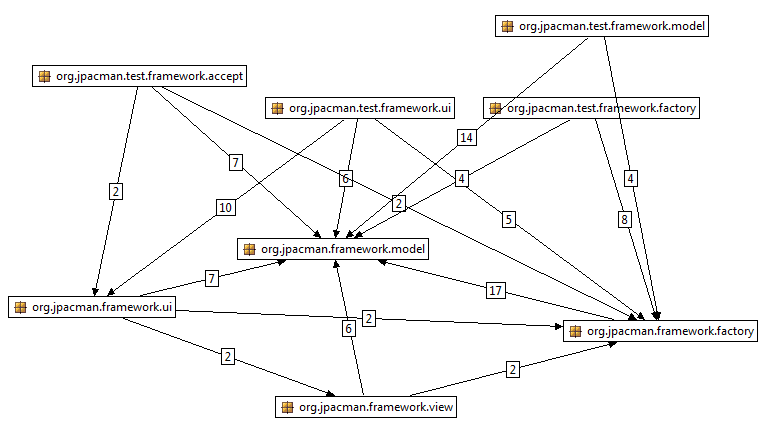
\includegraphics[width=\textwidth]{DependenciesPackages_refactor.png}
	\caption{\label{dependenciesPackage_refact}Détail de l'analyse des dépendences cycliques des packages du projet.}
\end{figure}

%%%%%%%%%%%%%%%%%%%%%%%%%%%%%%%%%%%%%%%%%%%%%%%%%%%%%%%%%%%%%%%%%%%%%%%%%%%%%%
\subsection{Code inutile}\label{deadCode_refact}
Ces modifications sont subtile et n'ont pas grand intérêt ni valeur ajoutée, et tel que déjà sugéré lors de l'analyse (voir sous-section \ref{deadCode}), il n'y a finalement que peux de travail à effectuer ici.
Les packages de test, les variables "serialVersionUID", les fichiers "package-info.java",  sont important donc ne peuvent pas être modifiés.\\
Concrétement, ont été modifié : 
\begin{itemize}
\item un ";" a été supprimé dans le classe "...model.IBoardInspector" ;
\item une déclaration redondante dans la classe "...view.ImageLoader" et dans la classe "...factory.MapParser".
\end{itemize}


%%%%%%%%%%%%%%%%%%%%%%%%%%%%%%%%%%%%%%%%%%%%%%%%%%%%%%%%%%%%%%%%%%%%%%%%%%%%%%
\subsection{Javadoc}\label{javadoc_refact}
Comme précisé dans l'énoncé, le temps disponible est assez court donc ce critère a été évalué comme mineur. Certains ajout se feront peut-être mais au fur et à mesure du travail sur les autres missions mais pas façon systématique. En voici la liste : 

%%%%%%%%%%%%%%%%%%%%%%%%%%%%%%%%%%%%%%%%%%%%%%%%%%%%%%%%%%%%%%%%%%%%%%%%%%%%%%
\subsection{Test unitaire}\label{unitTest_refact}
Rien n'a été refactoré dans le package "src.test.java.org.jpacman.test.framework.*". mais suite à d'autres modification, 2 test ont été commenté suite à la suppression de 2 méthodes (withFactory() et withButtonPanel() ) dans la classe "MainUI".

%%%%%%%%%%%%%%%%%%%%%%%%%%%%%%%%%%%%%%%%%%%%%%%%%%%%%%%%%%%%%%%%%%%%%%%%%%%%%%
\subsection{Flux de conception}\label{designflaws_refact}
\begin{figure}[!h]
	\centering
	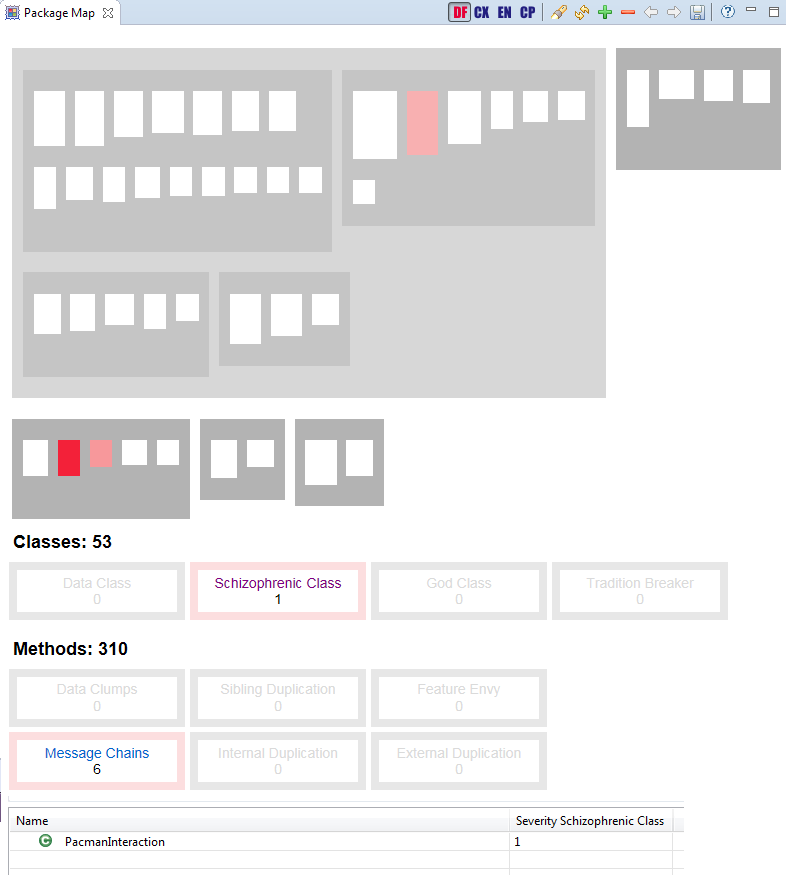
\includegraphics[width=\textwidth]{InCodeDesignFlaws_refactor.png}
	\caption{\label{designflaws_refact}Analyse de la structure du code par InCode.}
\end{figure}
En regardant la sévérité des classes schizophréniques, il est évident que la classe "Game" doit-être travaillée en priorité. Ce fut chose faite en déplaçant les méthodes "movePlyer()" et "moveGhost()" respectivement dans les classes "Player" et "Ghost". La \labelfigure{designflaws_refact} montre le résultat de se changement.\\
Pour l'autre classe, une première séparation a été faite entre la partie gestion des événements clavier et la partie interaction avec pacman en créant la classe PacmanInteractor. C'est donc maintenant cette dernière qui est répertoriée comme schizophréniques. Une seconde séparation est donc surement possible, mais le choix est de la garder tel qu'elle est. 

%%%%%%%%%%%%%%%%%%%%%%%%%%%%%%%%%%%%%%%%%%%%%%%%%%%%%%%%%%%%%%%%%%%%%%%%%%%%%%
\subsection{Complexité}
\begin{figure}[!h]
	\centering
	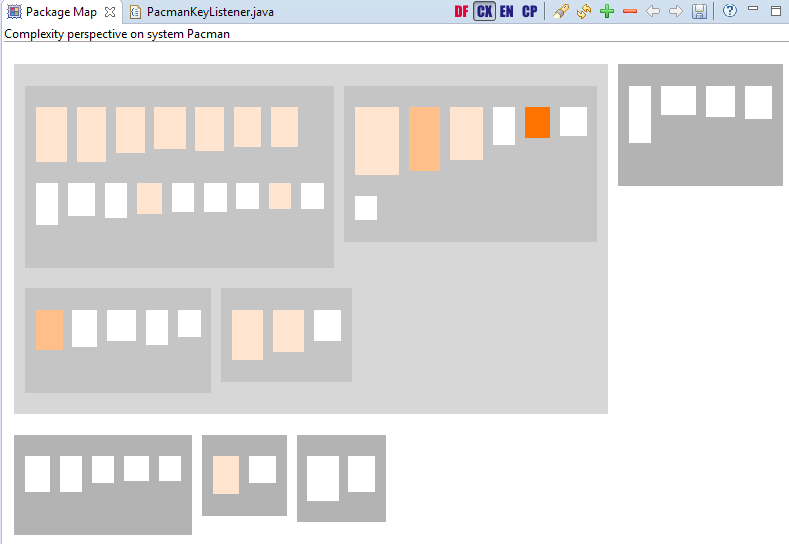
\includegraphics[width=\textwidth]{InCodeComplexity_refactor.png}
	\caption{\label{complexity_refact}Analyse de la complexité par InCode.}
\end{figure}
La \labelfigure{complexity_refact} permet de voir que la complexité est restée sur la classe "PacmanKeyListener". C'est dù au fait que dans l'une des méthodes se trouve un switch qui est composée de beaucoup de cas.

%%%%%%%%%%%%%%%%%%%%%%%%%%%%%%%%%%%%%%%%%%%%%%%%%%%%%%%%%%%%%%%%%%%%%%%%%%%%%%
\subsection{Encapsulation}
\begin{figure}[!h]
	\centering
	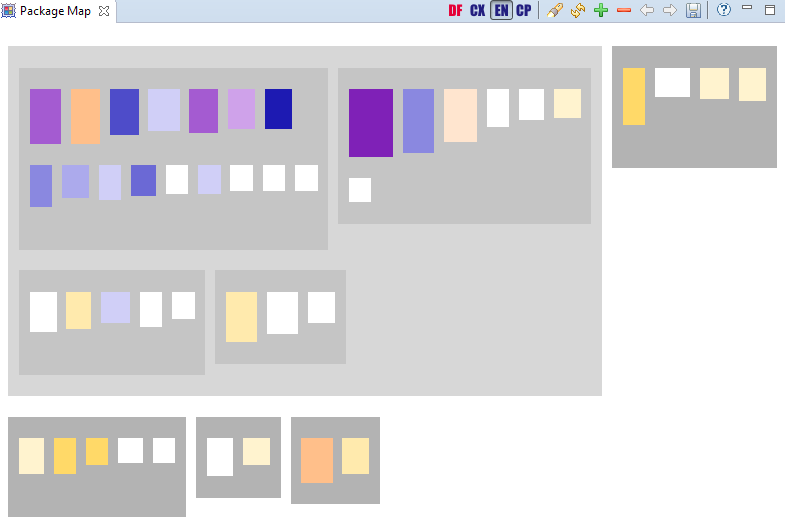
\includegraphics[width=\textwidth]{InCodeEncapsulation_refactor.png}
	\caption{\label{encapsulation_refact}Analyse de la complexité par InCode.}
\end{figure}
Aucun travail n'a réellement été réalisé sur ce critère, on remarque tout de même certaines modifications dont : 
\begin{itemize}
\item La classe "MainUI" s'est affirmée avec encore plus de clients.
\item La classe "Game" avait tendance à avoir plus de client et maintenant elle a plus de fournisseur.
\end{itemize}
%%%%%%%%%%%%%%%%%%%%%%%%%%%%%%%%%%%%%%%%%%%%%%%%%%%%%%%%%%%%%%%%%%%%%%%%%%%%%%
\subsection{Couplage}
\begin{figure}[!h]
	\centering
	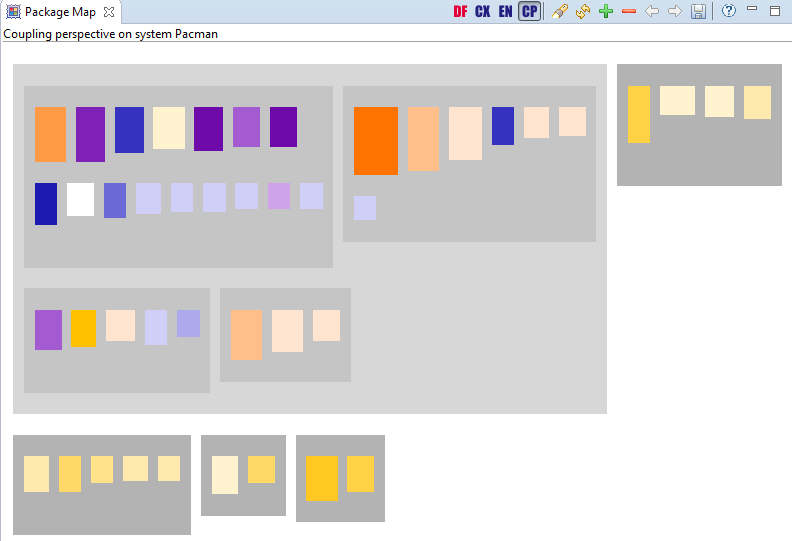
\includegraphics[width=\textwidth]{InCodeCoupling_refactor.png}
	\caption{\label{coupling_refact}Analyse de la complexité par InCode.}
\end{figure}
La \labelfigure{coupling_refact} nous montre, comparé à la \labelfigure{coupling}, que il n'y a pas eu de gros changement de ce côté-là.

%%%%%%%%%%%%%%%%%%%%%%%%%%%%%%%%%%%%%%%%%%%%%%%%%%%%%%%%%%%%%%%%%%%%%%%%%%%%%%
\subsection{Pyramide des métriques}
\begin{figure}[!h]
	\centering
	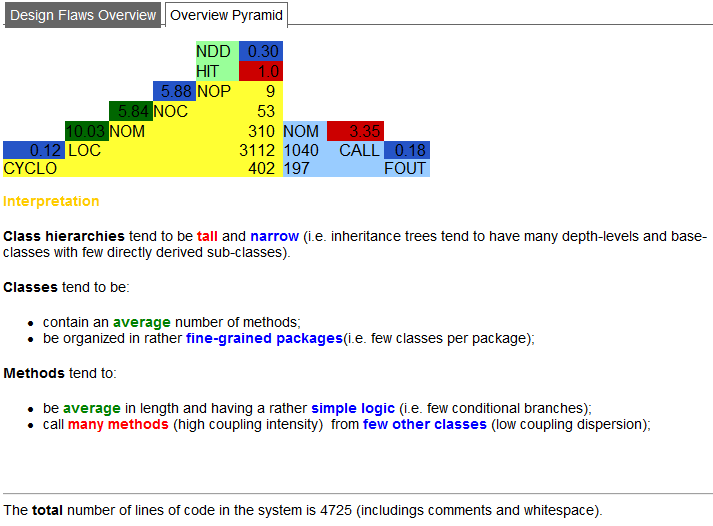
\includegraphics[width=\textwidth]{InCodePyramid_refactor.png}
	\caption{\label{pyramid_refact}Pyramide des valeurs calculées par InCode.}
\end{figure}
La \labelfigure{pyramid_refact} montre que la seule différence significative est que l'arbre que constitue les classe s'est élargit.\\

\clearpage
%%%%%%%%%%%%%%%%%%%%%%%%%%%%%%%%%%%%%%%%%%%%%%%%%%%%%%%%%%%%%%%%%%%%%%%%%%%%%%
\subsection{Métriques}
\begin{figure}[!h]
	\centering
	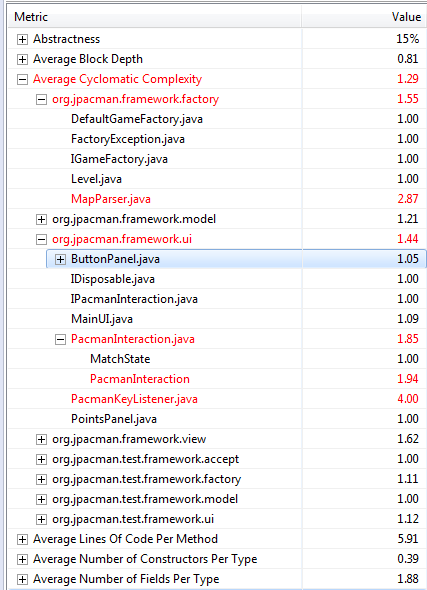
\includegraphics[height=\textheight]{Metrique3.png}
	\caption{\label{métrique3}Détails de l'analyse des métriques du projet (partie 1).}
\end{figure}
\begin{figure}[!h]
	\centering
	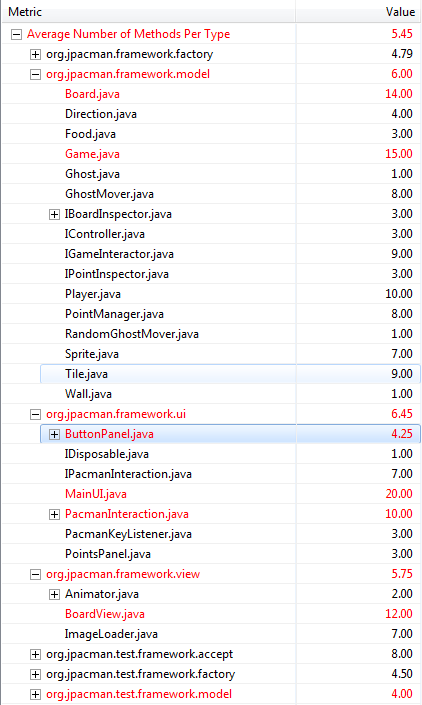
\includegraphics[height=\textheight]{Metrique4.png}
	\caption{\label{métrique4}Détails de l'analyse des métriques du projet (partie 2).}
\end{figure}
\begin{figure}[!h]
	\centering
	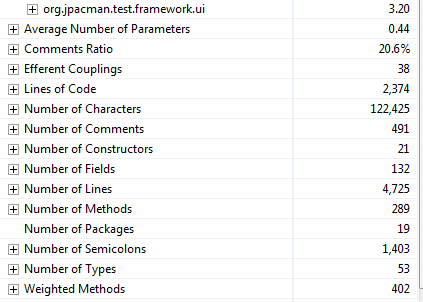
\includegraphics[width=\textwidth]{Metrique5.png}
	\caption{\label{métrique5}Détails de l'analyse des métriques du projet (partie 3).}
\end{figure}

Suite au refactoring du code dupliqué, on observe que le nombre de problème n'a pas vraiment diminué. Certains cas ont été déplacé, mais c'est tout.

\clearpage
%%%%%%%%%%%%%%%%%%%%%%%%%%%%%%%%%%%%%%%%%%%%%%%%%%%%%%%%%%%%%%%%%%%%%%%%%%%%%%
\subsection{Audit}
Cet intitulé reprend tous les problèmes et les erreurs de code tel que les erreurs non capturées, la sérialisation les imports inutiles, les droit d'accès,...\\
Voici celles détectées par l'outil CodePro d'Eclipse : 
\begin{figure}[!h]
	\centering
	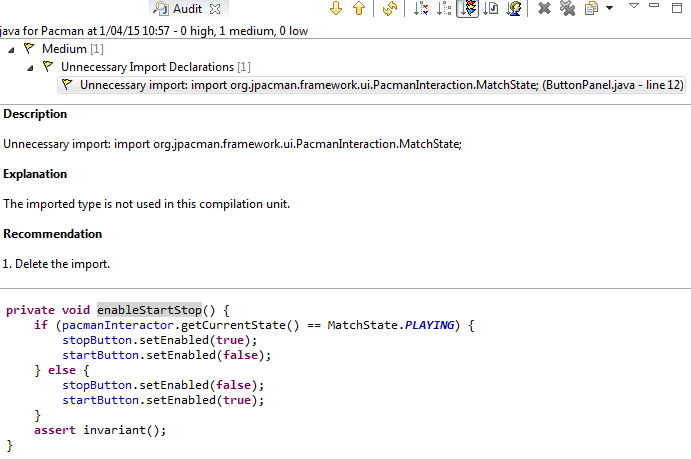
\includegraphics[width=\textwidth]{Audit_refactor.png}
	\caption{\label{Audit_refact}Détail de l'analyse d'audit faite par Eclipse.}
\end{figure}

\subsubsection{Import inutile}
Un seul import reste dans l'analyse. La justification est que lors de sa suppression, une erreur est signalée au niveau de la fonction illustrée dans le bas de l'image.

%%%%%%%%%%%%%%%%%%%%%%%%%%%%%%%%%%%%%%%%%%%%%%%%%%%%%%%%%%%%%%%%%%%%%%%%%%%%%%
\subsection{Conclusion}
Après ces quelques heures de travail, il est évident que il y a un mieux, cependant, il n'est pas significatif.


%%%%%%%%%%%%%%%%%%%%%%%%%%%%%%%%%%%%%%%%%%%%%%%%%%%%%%%%%%%%%%%%%%%%%%%%%%%%%%%%%%
\newpage
\section{Etape 5 : Extensions}\label{sec:etape5}

Maintenant que le logiciel a été étudié, réparer, réétudié, on peut commencer à l'améliorer et à ajouter de nouvelles fonctionnalités.
%Utilisez un processus de développement dirigé par les tests (test-driven development) : lors du développement des extensions, ajoutez de nouveaux tests unitaires pour tester le comportement prévu de l'extension. Effectuez également des tests de régression avec les tests unitaires déjà présents, afin de vous assurer que le comportement initial n'a pas été modifié.
\subsection{IA fantômes} 
\subsubsection{Règle}
Actuellement, le comportement des fantômes est assez erratique, car la direction empruntée par chacun d'eux est déterminée aléatoirement. Commencez par attribuer une couleur à chacun des quatre fantômes du jeu, afin que le joueur puisse les difféerencier. Créez des IA pour les fantômes afin qu'ils prennent des décisions
plus intéressantes pour le joueur. Une décision de direction n'est prise que lorsqu'un fantôme arrive à un embranchement. La décision est basée sur le calcul de la plus courte distance entre la position de case de l'embranchement et la position que le fantôme souhaite atteindre. Si plusieurs directions sont pareillement préférables, un fantôme préférera toujours aller en haut, puis à gauche, puis en bas. Un fantôme ne peut donc aller à droite que si cette direction est la seule représentant la plus petite distance jusqu'à la destination.\\
Le comportement des fantômes alterne entre un mode de \textbf{poursuite} et un mode de \textbf{dispersion}.\\
En mode poursuite, chaque fantôme a un comportement et une vitesse spécifiques et déeterministes\footnote{http://gameinternals.com/post/2072558330/understanding-pac-man-ghost-behavior} :
\begin{itemize}
\item \textbf{Blinky} a une philosophie très simple : "Droit au but ! ". En toute circonstance, il tente de se rendre
sur la case où se trouve Pac-Man par le chemin le plus court. Il a une vitesse de déplacement de $100\%$.
\item \textbf{Pinky} aime tendre des embuscades. Il devine où sera Pac-Man $4$ mouvements plus tard et se rend à
cette position. Il a une vitesse de déplacement de $80\%$.
\item \textbf{Inky} est dificilement prévisible pour un humain, car son comportement dépend des positions et des
directions de Pac-Man et de Blinky. Imaginez un vecteur joignant la position de Blinky à celle où
se trouvera Pac-Man dans $2$ mouvements. Doublez la longueur de ce vecteur. La position que Inky
cherche à atteindre est à l'extrémité de ce vecteur. Il a une vitesse de déplacement de $100\%$.
\item \textbf{Clyde} ne semble pas se préoccuper des autres. Il a en fait deux modes de fonctionnement, et il passe de l'un à l'autre en fonction de la distance existant entre Pac-Man et lui. S'il se trouve à plus de $8$
cases de Pac-Man, Clyde a le même comportement que Blinky. Dans le cas contraire, il se rend sur la
case située dans le coin inférieur gauche du labyrinthe. Il a une vitesse de déplacement de $100\%$.
\end{itemize}
En mode dispersion, chaque fantôome se dirige vers sa position "maison". Ces positions sont situées aux quatre coins du labyrinthe :
\begin{itemize}
\item Blinky se rend dans le coin supérieur droit.
\item Pinky se rend dans le coin supérieur gauche.
\item Inky se rend dans le coin inférieur droit.
\item Clyde se rend dans le coin inférieur gauche.
\end{itemize}
Une fois sa position "maison" atteinte, le fantôme va se déplacer dans un circuit qui consiste à toujours emprunter le chemin de gauche pour Pinky et Clyde, et celui de droite pour Blinky et Inky (cf. \labelfigure{ghostdispersion})
\begin{figure}[!h]
	\centering
	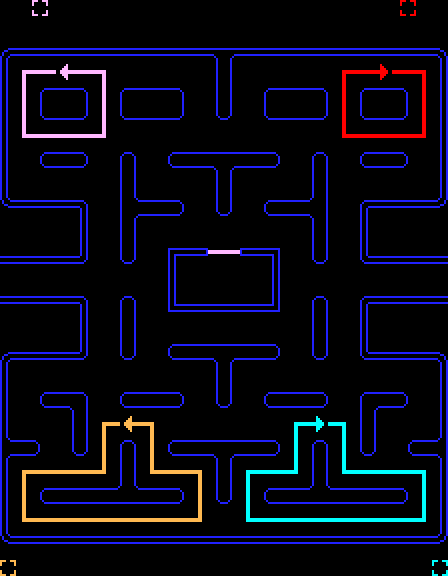
\includegraphics[width=\textwidth]{pacman_ghostmove_dispersion.png}
	\caption{\label{ghostdispersion}Circuits empruntés par les fantômes en mode dispersion.}
\end{figure}
L'alternance entre ces modes est définie comme suit :
\begin{itemize}
\item Dispersion pendant 7 secondes, puis poursuite pendant 20 secondes.
\item Dispersion pendant 7 secondes, puis poursuite pendant 20 secondes.
\item Dispersion pendant 5 secondes, puis poursuite pendant 20 secondes.
\item Dispersion pendant 5 secondes, puis poursuite indéfiniment.
\end{itemize}
%Utilisez un Strategy Design Pattern pour implémenter les comportements des fantômes. L'alternance entre la dispersion et la poursuite sera ainsi réalisée grâce à un changement de stratégie. De même, les aspects communs des comportements des fantômes seront implémentés sous la forme de stratégies partagées par les antagonistes concernés.
%Le système doit être tel que l'ajout de nouvelles stratégies soit possible et facile : les stratégies doivent avoir toutes les informations nécessaires pour agir en état de cause. En aucune manière, les stratégies ne doivent pouvoir tricher en manipulant les données du jeu ou en donnant des instructions contraires aux règles du jeu.

\subsubsection{Implémentation}






%%%%%%%%%%%%%%%%%%%%%%%%%%%%%%%%%%%%%%%%%%%%%%%%%%%%%%%%%%%%%%%%%%%%%%%%%%%%%%%%%%%%%%%%%%%%%%%%%%%%%
\subsection{Super gommes}
\subsubsection{Règle}
Modifiez le jeu afin qu'il prenne en compte la présence de supergommes. Lorsque Pac-Man mange une supergomme, elle lui rapporte $50$ points.\\
Pendant un court moment, les règles du jeu changent (le jeu se met en mode fuite) et la proie devient chasseur. Lorsque Pac-Man mange une supergomme, les fantômes sont effrayés. Le chronomètre du mode dans lequel ils se trouvent s'arrête et les fantômes entrent en mode fuite : ils deviennent bleus et leur vitesse de déplacement est réduite à $50\%$ (y compris pour Pinky). En mode fuite, chaque fantôme décide aléatoirement
de la direction à prendre à chaque embranchement. Si Pac-Man touche un fantôme en mode fuite, celui-ci disparaît du jeu et réapparaît au milieu du labyrinthe après $5$ secondes.\\
Si Pac-Man touche un fantôme en mode fuite, il le mange, ce qui lui rapporte :
\begin{itemize}
\item $200$ points pour le premier fantôme mangé;
\item $400$ points pour le second fantôme mangé;
\item $800$ points pour le troisième fantôme mangé;
\item $1600$ points pour le quatrième fantôme mangé.
\end{itemize}
Il y a quatre supergommes par niveau. Les deux premiéres à être avalées effraient les fantômes pendant $7$ secondes, tandis que les deux dernières les effraient pendant $5$ secondes. Après ce délai, les fantômes retournent dans le mode dans lequel ils étaient avant de fuir. Le chronomètre associè à ce mode est repris là où il s'était arrêté.\\

\subsubsection{Implémentation}








%%%%%%%%%%%%%%%%%%%%%%%%%%%%%%%%%%%%%%%%%%%%%%%%%%%%%%%%%%%%%%%%%%%%%%%%%%%%%%%%%%
\newpage
\section{Etape 6 : Analyse de la qualité du logiciel}\label{sec:etape6}
\subsection{Enoncé} 
Pour chaque extension ajoutée, réalisez une analyse de qualité similaire à celle décrite en Section ... Au vu de cette analyse, quels sont les points qui devraient à présent être améliorés ?
\subsection{Résultat}



%%%%%%%%%%%%%%%%%%%%%%%%%%%%%%%%%%%%%%%%%%%%%%%%%%%%%%%%%%%%%%%%%%%%%%%%%%%%%%%%%%
\newpage
\section{Etape 7 : Analyse de l'évolution de la qualité logicielle}\label{sec:etape7}
\subsection{Enoncé} 
Analysez l'évolution de la qualité du logiciel entre les différentes versions, en utilisant les résultats d'analyse de qualité des sections ..., ... et ... . Montrez cette évolution graphiquement et interprètez-la.
\subsection{Résultat}

%%%%%%%%%%%%%%%%%%%%%%%%%%%%%%%%%%%%%%%%%%%%%%%%%%%%%%%%%%%%%%%%%%%%%%%%%%%%%%%%%%
\clearpage
\newpage
\section{Annexes} \label{sec:annexe}
\appendix %permet de changer la numérotation en lettre
\section{Annexe : Code Dupliqué}\label{SimilarCode}
Dans cette section se trouve les différentes annexes qui permettent d'identifier les blocs de code dupliqués détectés par CodePro. Chaque image illustre un bloc de code mis à part la dernière qui illustre les 6 derniers blocs de code et est issue du rapport généré par CodePro (parce que Eclipse les masque).
N.B. : La figure reprenant tous les blocs identifiés se trouve à la sous-section \ref{codeduplique}
\subsubsection{Avant refactoring}
\begin{figure}[ht]
	\centering
	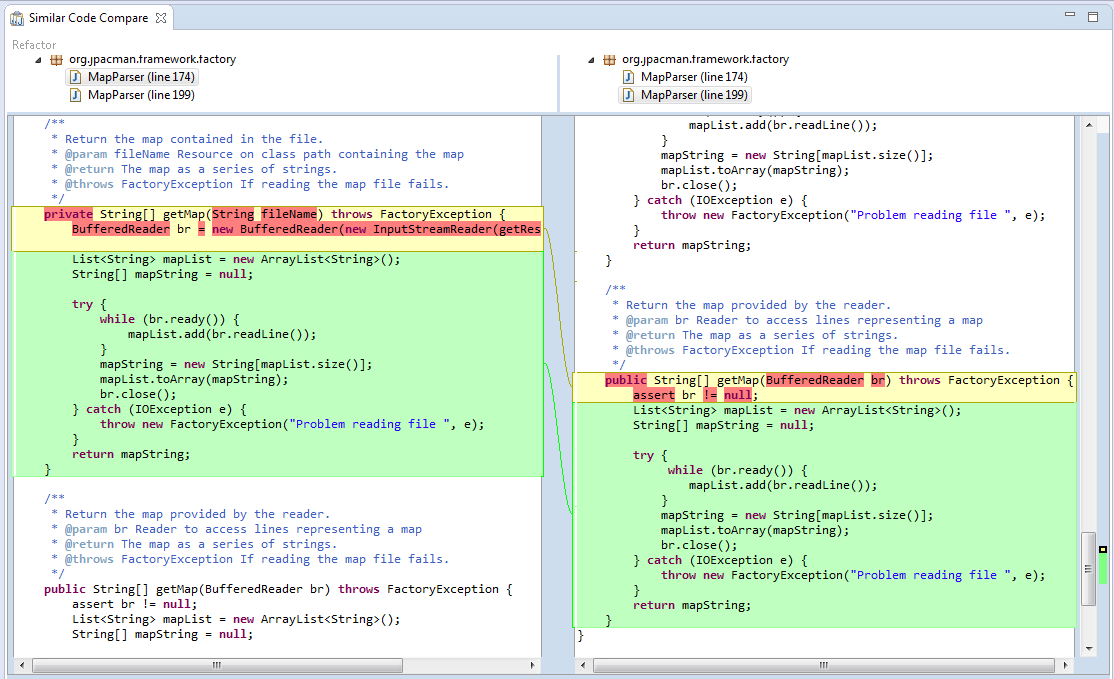
\includegraphics[width=\textwidth]{images/SimilarCode_1.png}
	\caption{\label{SimilarCode1}Détail de l'analyse de code redondant par CodePro}
\end{figure}

\begin{figure}[ht]
	\centering
	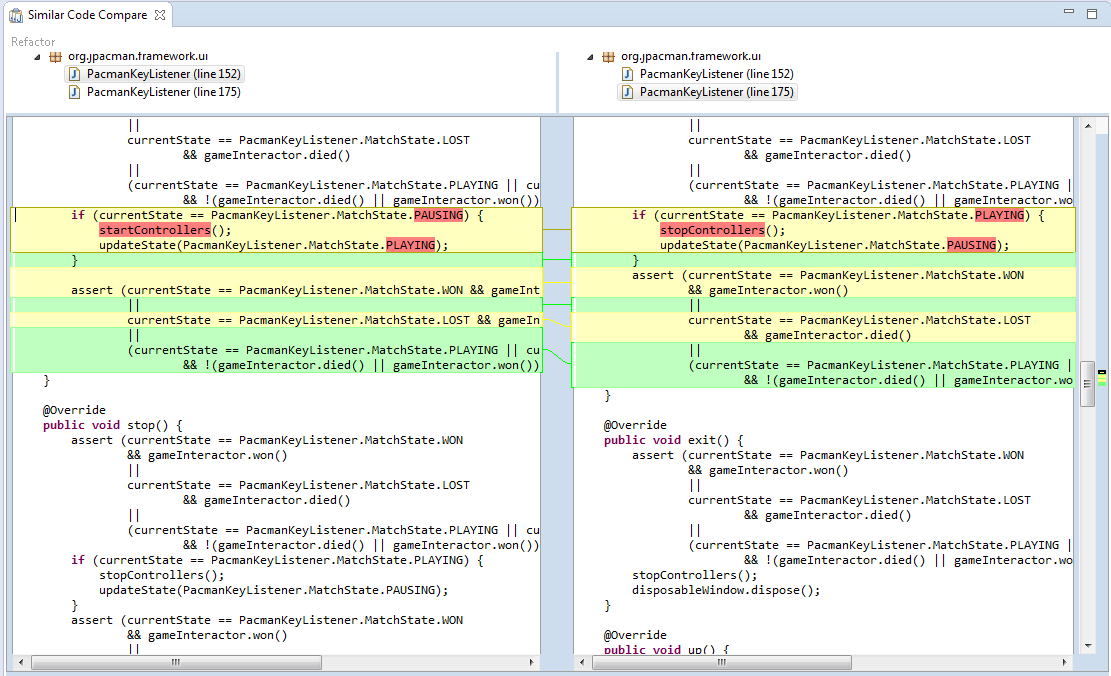
\includegraphics[width=\textwidth]{images/SimilarCode_2.png}
	\caption{\label{SimilarCode2}Détail de l'analyse de code redondant par CodePro}
\end{figure}

\begin{figure}[ht]
	\centering
	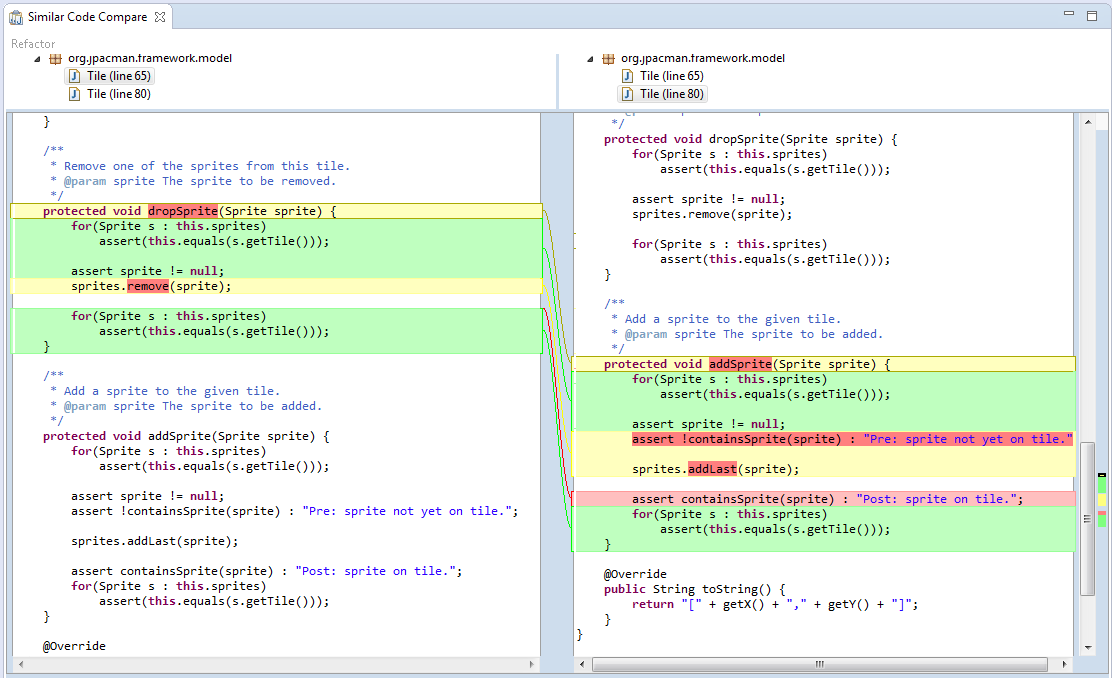
\includegraphics[width=\textwidth]{images/SimilarCode_3.png}
	\caption{\label{SimilarCode3}Détail de l'analyse de code redondant par CodePro}
\end{figure}

\begin{figure}[ht]
	\centering
	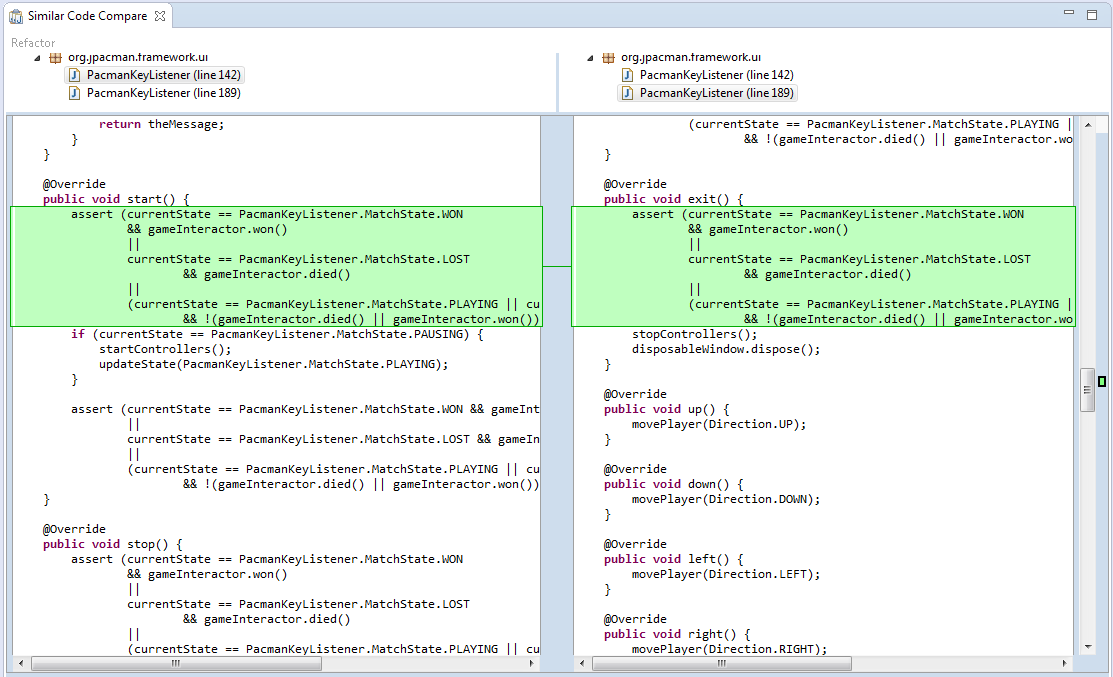
\includegraphics[width=\textwidth]{images/SimilarCode_4.png}
	\caption{\label{SimilarCode4}Détail de l'analyse de code redondant par CodePro}
\end{figure}

\begin{figure}[ht]
	\centering
	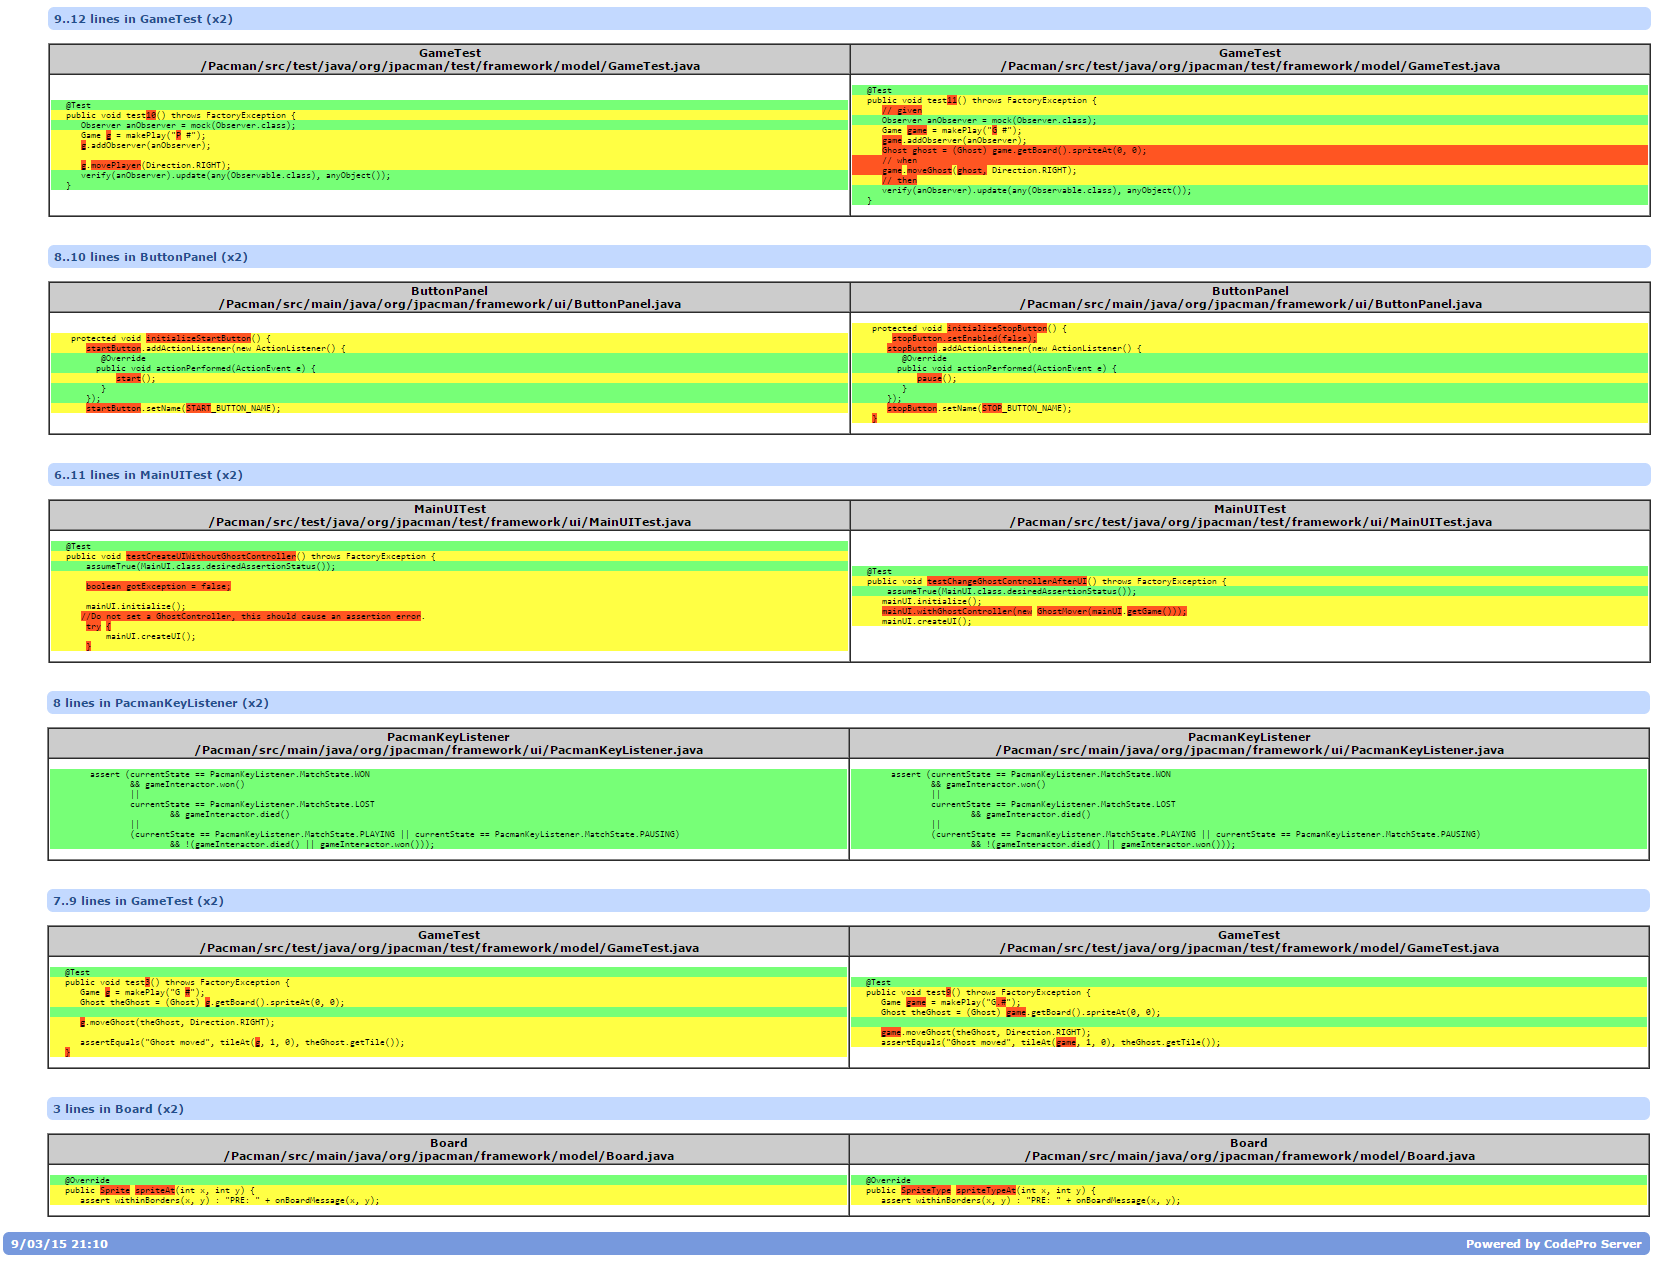
\includegraphics[width=\textwidth]{images/SimilarCode_5.png}
	\caption{\label{SimilarCode5}Détail de l'analyse de code redondant par CodePro (élément dont la visualisation n'est pas possible dans Eclipse)}
\end{figure}

\subsubsection{Après refactoring}
\begin{figure}[ht]
	\centering
	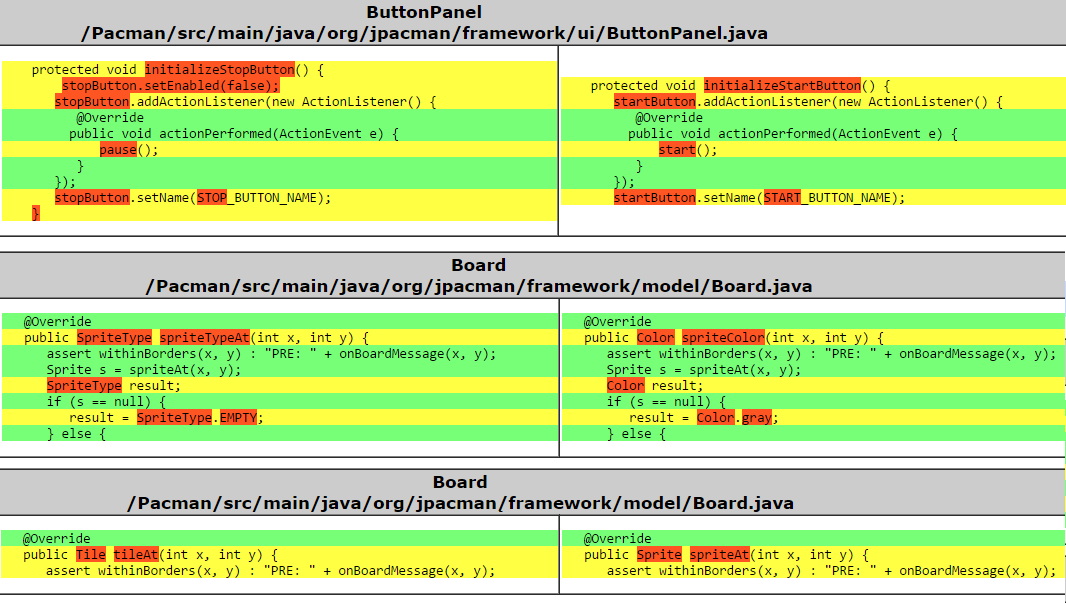
\includegraphics[width=\textwidth]{images/SimilarCode_7.png}
	\caption{\label{SimilarCode7}Détail de l'analyse de code redondant par CodePro}
\end{figure}

\clearpage
\newpage
\section{Annexe : Dépendances}\label{Dependencies}
Ces figures permettent de visualiser les dépendances entre les différents éléments du projet.
N.B. : Les figures des dépendances entre les packages et des dépendances au sein du package Model se trouvent à la sous-section \ref{dépendances}.

\begin{figure}[ht]
	\centering
	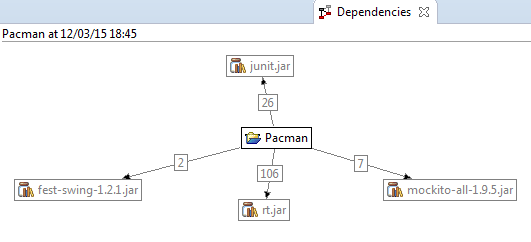
\includegraphics[width=\textwidth]{images/DependenciesProject.png}
	\caption{\label{dependenciesP}Détail de l'analyse des dépendences cycliques du projet.}
\end{figure}

\begin{figure}[ht]
	\centering
	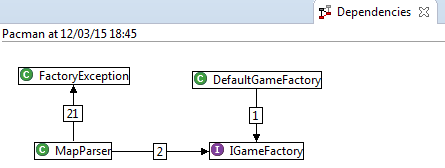
\includegraphics[width=\textwidth]{images/DependenciesFactory.png}
	\caption{\label{dependenciesF}Détail de l'analyse des dépendences cycliques du package Factory.}
\end{figure}

\begin{figure}[ht]
	\centering
	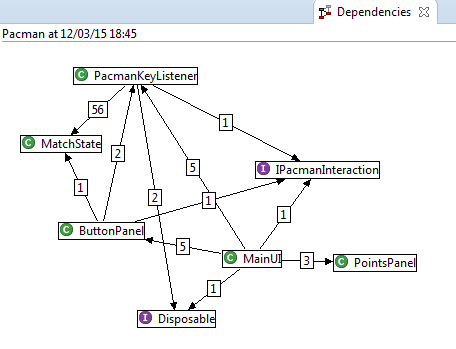
\includegraphics[width=\textwidth]{images/DependenciesUI.png}
	\caption{\label{dependenciesUI}Détail de l'analyse des dépendences cycliques du package UI.}
\end{figure}

\begin{figure}[ht]
	\centering
	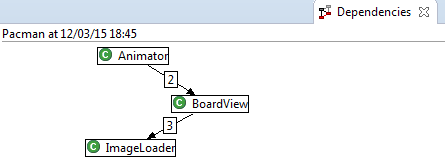
\includegraphics[width=\textwidth]{images/DependenciesVieuw.png}
	\caption{\label{dependenciesV}Détail de l'analyse des dépendences cycliques du package Vieuw.}
\end{figure}

\begin{figure}[ht]
	\centering
	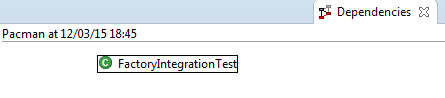
\includegraphics[width=\textwidth]{images/DependenciesFactoryTest.png}
	\caption{\label{dependenciesFT}Détail de l'analyse des dépendences cycliques du package Factory (Test).}
\end{figure}

\begin{figure}[ht]
	\centering
	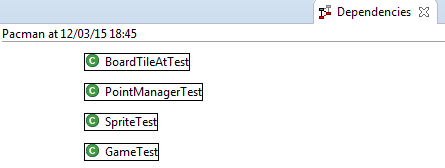
\includegraphics[width=\textwidth]{images/DependenciesModelTest.png}
	\caption{\label{dependenciesMT}Détail de l'analyse des dépendences cycliques du package Model (Test).}
\end{figure}

\begin{figure}[ht]
	\centering
	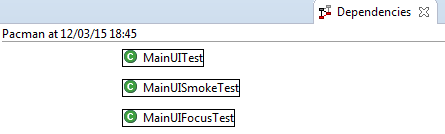
\includegraphics[width=\textwidth]{images/DependenciesUITest.png}
	\caption{\label{dependenciesUIT}Détail de l'analyse des dépendences cycliques du package UI (Test).}
\end{figure}

\begin{figure}[ht]
	\centering
	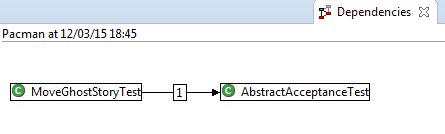
\includegraphics[width=\textwidth]{images/DependenciesAcceptTest.png}
	\caption{\label{dependenciesAT}Détail de l'analyse des dépendences cycliques du package Accept (Test).}
\end{figure}

\begin{figure}[ht]
	\centering
	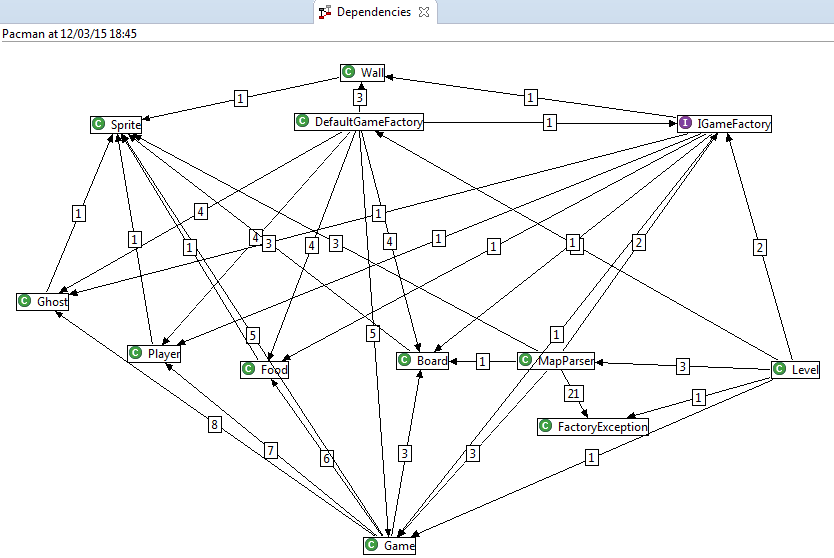
\includegraphics[width=\textwidth]{images/DependenciesModel_Factory.png} %images/DependenciesModel_Factory1.png
	\caption{\label{dependenciesMF}Détail de l'analyse des dépendences cycliques entre le package Model et la package Factory.} %avec en gras les classes du package Factory
\end{figure}


\clearpage
\newpage
\section{Annexe : Incode}\label{InCode}

\begin{figure}[ht]
	\centering
	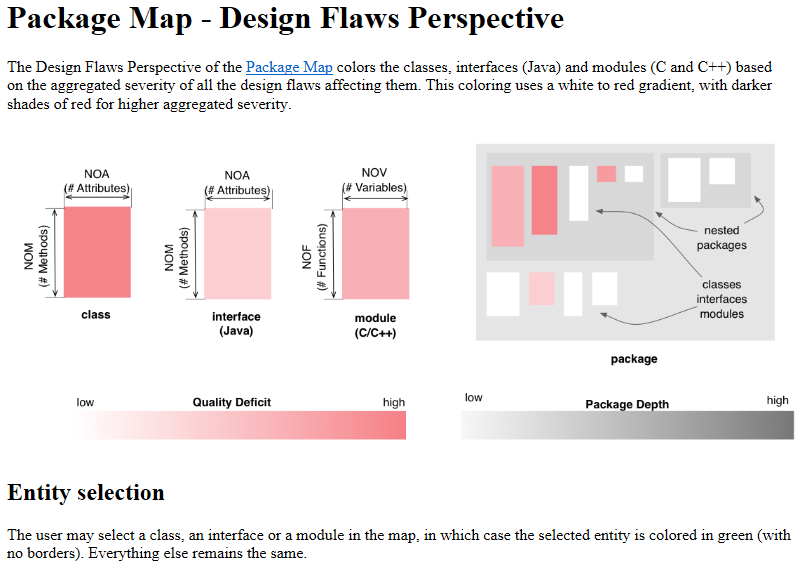
\includegraphics[width=\textwidth]{images/InCodeDesignFlawsLegende.png}
	\caption{\label{designflawsLeg}Légende de l'outil InCode d'analyse de conception}
\end{figure}

\begin{figure}[ht]
	\centering
	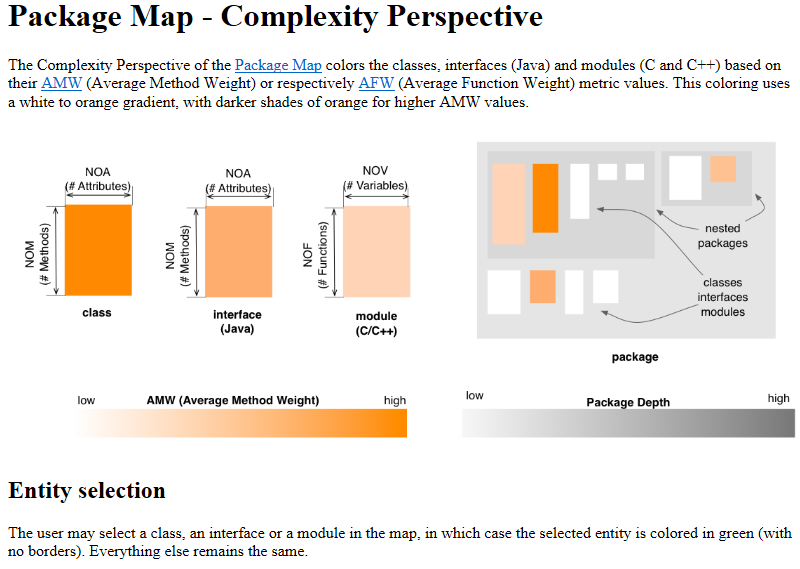
\includegraphics[width=\textwidth]{images/InCodeComplexityLegende.png}
	\caption{\label{complexityLeg}Légende de l'outil InCode d'analyse de complexité}
\end{figure}

\begin{figure}[ht]
	\centering
	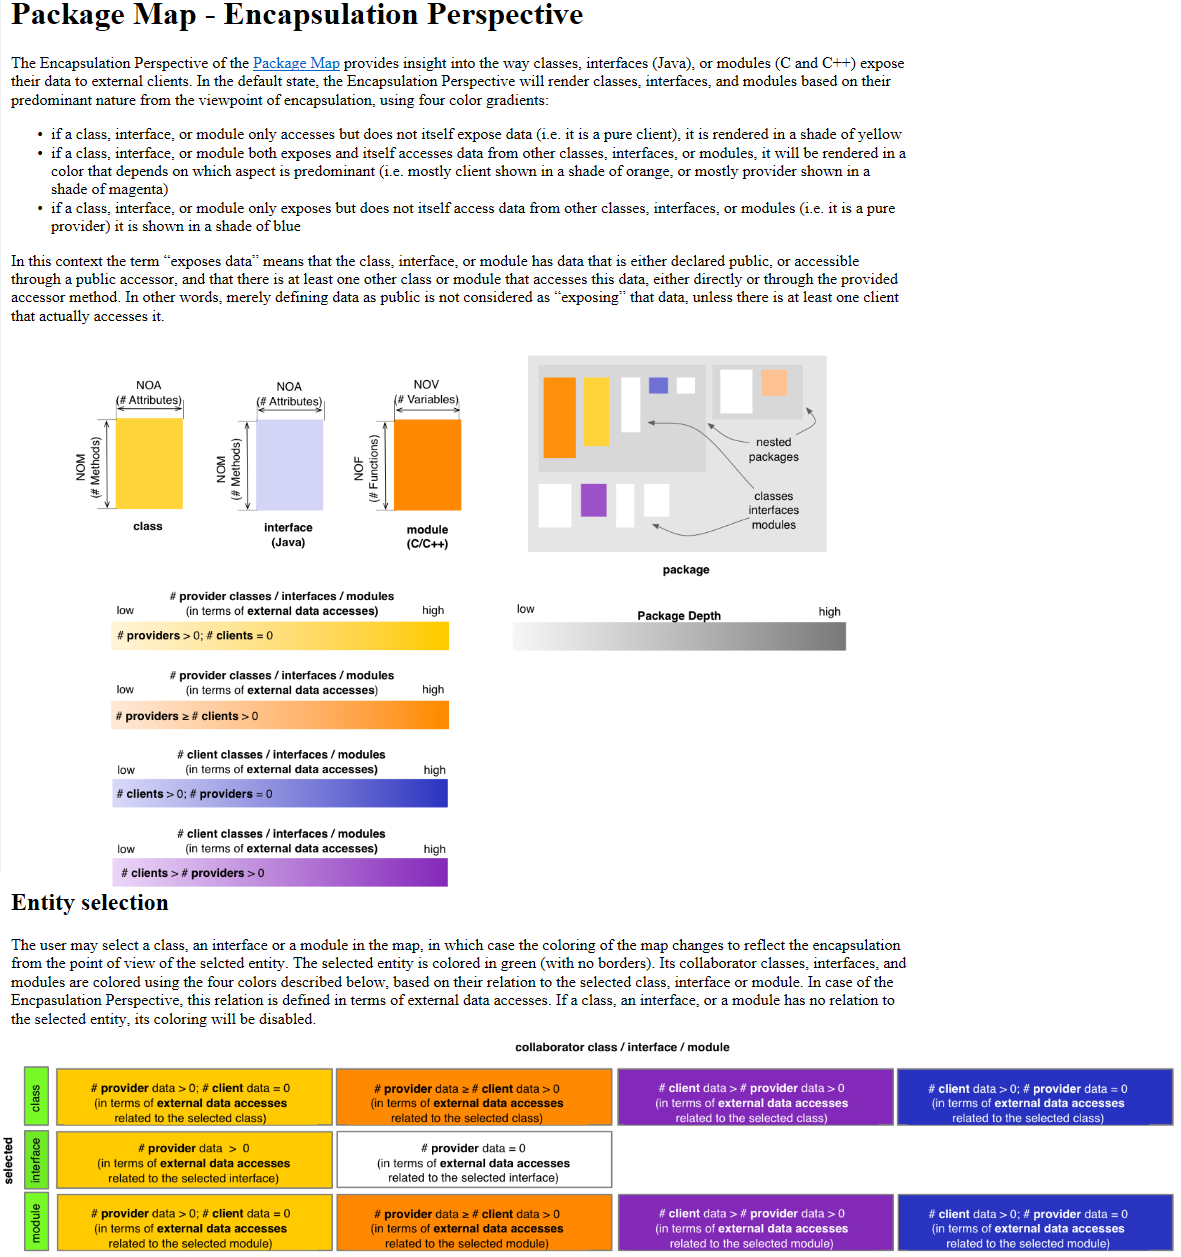
\includegraphics[width=\textwidth]{images/InCodeEncapsulationLegende.png}
	\caption{\label{encapsulationLeg}Légende de l'outil InCode d'analyse d'encapsulation}
\end{figure}

\begin{figure}[ht]
	\centering
	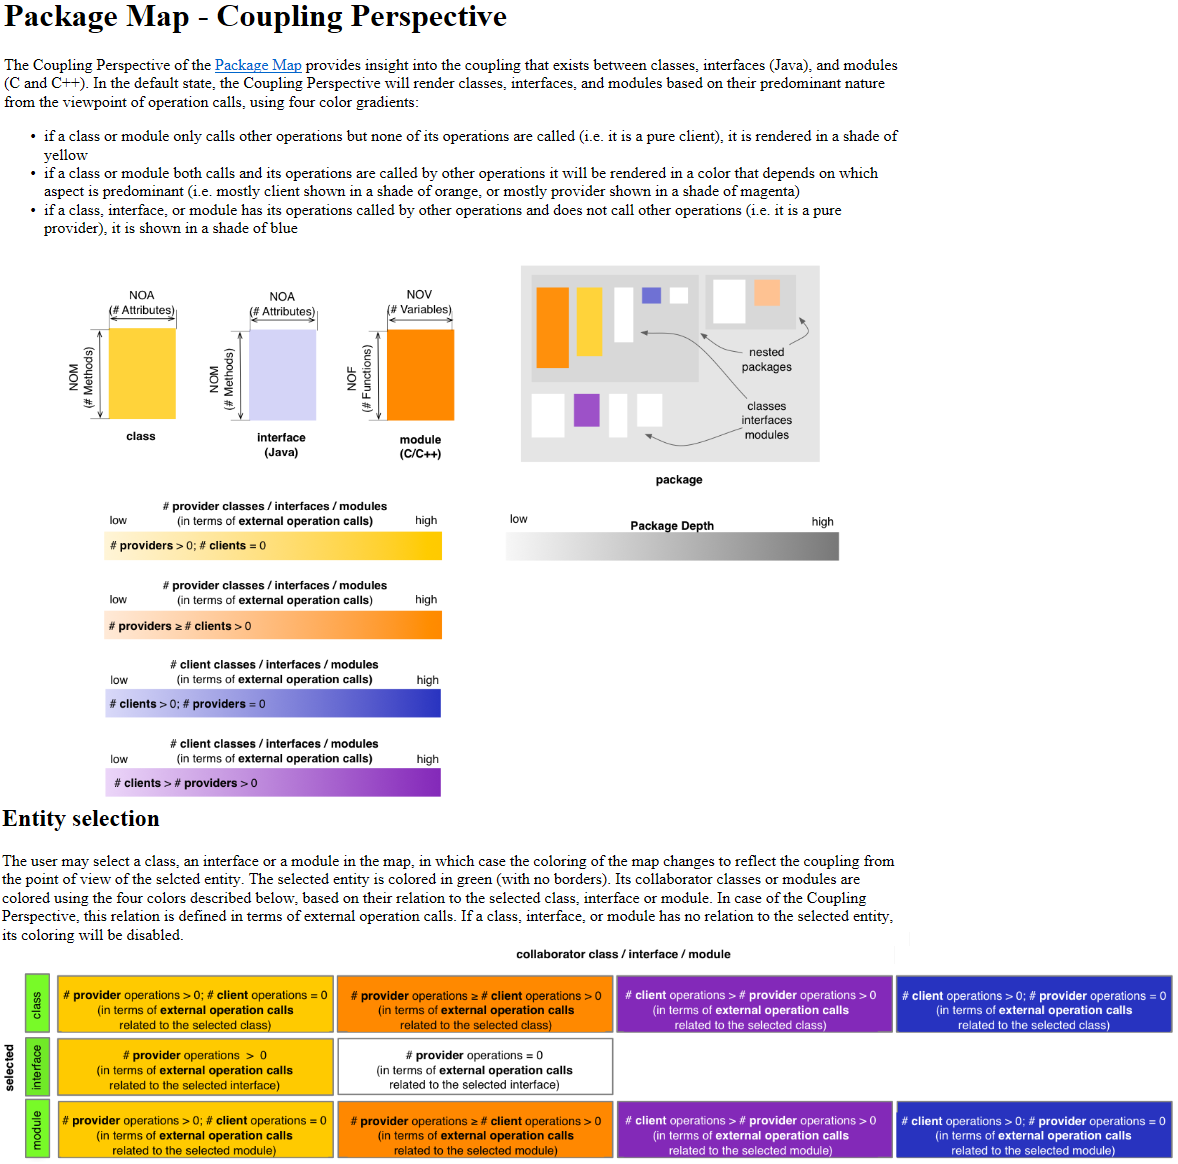
\includegraphics[width=\textwidth]{images/InCodeCouplingLegende.png}
	\caption{\label{couplingLeg}Légende de l'outil InCode d'analyse de couplage}
\end{figure}

\begin{figure}[ht]\label{pyramidLeg}
L'Aperçu Pyramide rassemble en un seul endroit les mesures les plus importantes sur un système orienté objet. Il se compose de trois parties, chacune quantifie un aspect important de la conception de systèmes orientés objet : la taille et la complexité, l'utilisation de l'héritage, et le couplage.

Le côté gauche de la pyramide aperçu (zone jaune) fournit des informations caractérisant la taille et la complexité du système. Ils comptent les unités les plus importantes de la modularité d'un système orienté objet, du plus haut niveau, jusqu'aux plus basses unités de mesures : 
• NOP (nombre total de packages définis dans le système);
• CNP ou NOC (nombre total de classes définies dans le système, sans compter les classes de la bibliothèque);
• NOM (nombre total de méthodes définies dans le système, y compris les méthodes et fonctions globales);
• LOC (nombre total de lignes de code appartenant à l'exploitation);
• CYCLO (somme des nombres cyclomatiques de toutes les opérations définies dans le système).
Les chiffres indiqués à la gauche de ces paramètres sont calculés par un rapport entre les mesures directement placés en dessous et à droite. où par exemple le rapport NOM / CNP représente le nombre moyen de méthodes dans une classe.

La partie supérieure de la pyramide (la zone verte) est dédié à l'utilisation de l'héritage : 
• NDD (nombre moyen de descendants directs d'une classe, à l'exclusion des classes de la bibliothèque. Si une classe n'a pas de classes dérivées, alors la classe participe avec une valeur de 0);
• HIT (moyenne de la métrique de HIT( = la longueur de trajet maximal d'une classe à sa plus profonde sous-classe) sur toutes les classes définies dans le système. Les classes autonomes sont considérés classes racines avec HIT = 0).

Le côté droit de la pyramide (la zone bleue) est dédié à l'aspect de couplage :
• CALL (nombre total d'opérations distinctes d'appelle dans le système);
• FOUT (somme de la métrique de FANOUT pour toutes les opérations définies dans le système)

Pour chaque rapport calculé, trois seuils sont calculés:
• faible - bleu
• Moyenne - vert
• haute - rouge
\end{figure}

\clearpage
\newpage
\section{Annexe : Couverture par les test}\label{coverage}

\begin{figure}[ht]
	\centering
	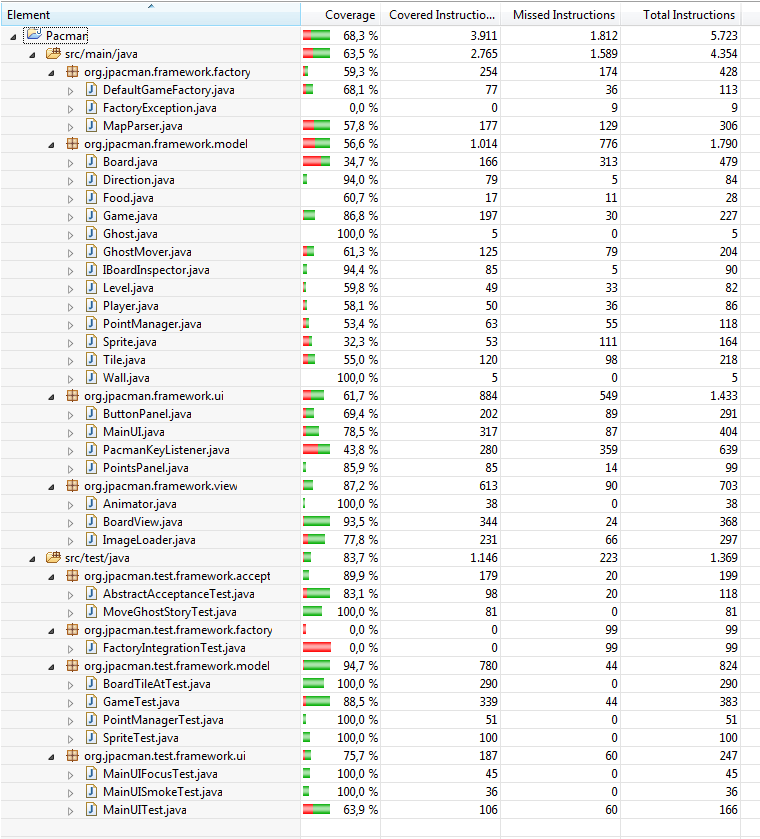
\includegraphics[width=\textwidth]{images/CoverageTest.png}
	\caption{\label{CoverageTest}Détail de l'analyse de couverture du code par les tests unitaires.}
\end{figure}





\newpage
\bibliographystyle{plain}
\bibliography{reference}

\end{document} 

